\documentclass[]{report}

\usepackage{psfrag}
\usepackage{amsmath}
\usepackage{amssymb}
\usepackage{pstricks, pst-node, pst-plot, pst-circ}
\usepackage{moredefs}
\usepackage{hyperref}
\usepackage{cleveref}
\usepackage{graphicx}
\usepackage{epstopdf}
\usepackage{epsfig}
\usepackage{algorithm}
\usepackage{program}

% Title Page
\title{ Homework 3-4 Solution \\ \centering of \\ \centering Optimization in Engineering Class\\ \centering (MECH601)}
\author{MSc. Burak ER}

\begin{document}
\maketitle

\begin{abstract}
Solved problems in this homework are some of the problems at the end of chapter 4, 10 and 11 of the book Introduction to Optimum Design by Jasbir Arora\cite{arora2004introduction}. The solution include the following problems; Problem 4.7, 4.9, 4.22, 4.32, 4.47, 4.60, 4.85, 4.101, 4.138, 4.150, 10.11, 10.16, 10.27, 10.53, 10.59, 10.68, 11.10, 11.12, 11.33.
\end{abstract}
\subsection*{Problem 4.7}
Write down the Taylor Series representation of $e^x$ including quadratic terms around $x^*=2$.
\subsubsection*{Solution}
Taylor series of any function around $x_0$ is given by
\begin{eqnarray}
f\left(x_0+\Delta x\right)&=&x_0+f^\prime\left(x_0\right)\Delta x+\frac{f^{\prime \prime}\left(x\right)}{2!}\left(\Delta x\right)^2+\dots
\end{eqnarray}
by putting $\Delta x=x-x_0$ and neglecting the higher order terms, it is found that
\begin{eqnarray*}
f\left(x\right)&=&2+e^2\left(x-2\right)+\frac{e^2}{2!}\left(x-2\right)^2 \\
&=&2+e^2\left(\frac{x^2}{2}-x\right)
\end{eqnarray*}
Therefore, Taylor series of $e^x$ around the point $x^*=2$ is found as
\begin{eqnarray*}
f\left(x\right)&=& e^2\left(\frac{x^2}{2}-x\right)+2
\end{eqnarray*}
\subsection*{Problem 4.9}
Determine the nature of the following quadratic form.
\begin{eqnarray}
F\left(\mathbf{x}\right)&=&x_1^2+4x_1x_2+2x_1x_3-7x_2^2-6x_2x_3+5x_3^2
\label{eqproblem:4.9}
\end{eqnarray}
\subsubsection*{Solution}
The quadratic form of the equation can be written as
\begin{eqnarray*}
F\left(\mathbf{x}\right)&=&\mathbf{x}^T\mathbf{P}\mathbf{x}
\end{eqnarray*}
\begin{eqnarray*}
\mathbf{x}&=&\left[x_1 \  x_2 \  x_3\right]^T
\end{eqnarray*}
\begin{eqnarray*}
\mathbf{P}&=&\left[\begin{array}{ccc}
1& 4& 2 \\
0& -7& -6\\
0& 0& 5
\end{array}\right]
\end{eqnarray*}
we can now determine the definition of the matrix $\mathbf{P}$ by finding the eigen values of it.
\begin{eqnarray*}
\mathrm{det}\left(\mathbf{P}-\lambda \mathbf{I}\right)&=&\mathrm{det}\left(\left[\begin{array}{ccc}
1-\lambda& 4& 2 \\
0& -7-\lambda& -6\\
0& 0& 5-\lambda
\end{array}\right]\right)=0
\end{eqnarray*}
From this determinant eigen value equation is found as
\begin{eqnarray*}
\left(-1\right)^2\left(1-\lambda\right)\left(-7-\lambda\right)\left(5-\lambda\right)+\left(-1\right)^3\left(4\right)\left(0\right)\left(0\right)+\left(-1\right)^4\left(2\right)\left(0\right)\left(0\right)&=&0
\end{eqnarray*}
or
\begin{eqnarray*}
\left(1-\lambda\right)\left(-7-\lambda\right)\left(5-\lambda\right)&=&0
\end{eqnarray*}
The eigen values of the $\mathbf{P}$ are $\lambda_1=1$ , $\lambda_2=-7$ , $\lambda_3=5$, thus, it is indefinite because of having at least one negative eigen value. Therefore, the function in equation \ref{eqproblem:4.9} is not convex.
\subsection*{Problem 4.22}
Find the stationary points for the following function. Also, determine the local minimum, local maximum and inflection points.
\begin{eqnarray}
f\left(\mathbf{x}\right)&=&3x_1^2+2x_1x_2+2x_2^2+7
\label{eqproblem:4.22}
\end{eqnarray}
\subsubsection*{Solution}
The function is written in quadratic form as
\begin{eqnarray*}
f\left(\mathbf{x}\right)&=&\mathbf{x}^T\mathbf{P}\mathbf{x}+\mathbf{b}
\label{eqproblem:4.22}
\end{eqnarray*}
\begin{eqnarray*}
\mathbf{x}&=&\left[\ x_1 \  x_2 \ \right]^T
\end{eqnarray*}
\begin{eqnarray*}
\mathbf{P}&=&\left[\begin{array}{ccc}
3& 2 \\
0& 2\\
\end{array}\right]
\end{eqnarray*}
\begin{eqnarray*}
\mathbf{b}&=&\left[\ 0 \  7 \ \right]^T
\end{eqnarray*}
stationary points is of the function is found by setting it's variation to zero
\begin{eqnarray*}
\delta{ f \left(\mathbf{x}\right)} &=& 0 \\
&=& 2\delta{\mathbf{x}}^T\mathbf{P}\mathbf{x}
\end{eqnarray*}
by setting $\delta \mathbf{x}$ arbitrary it is found
\begin{eqnarray*}
\mathbf{P}\mathbf{x}=0
\end{eqnarray*}
Resulting two linear equations
\begin{eqnarray*}
6x_1+2x_2=0\\
4x_2=0
\end{eqnarray*}
$x_1$ and $x_2$ is found
\begin{eqnarray*}
x_1=0\\
x_2=0
\end{eqnarray*}
From the definition $\mathbf H=2\mathbf{P}$. The eigen values of $\mathbf H$;
\begin{eqnarray*}
\mathrm{det}\left(\mathbf{H}-\lambda \mathbf{I}\right)&=&\mathrm{det}\left(\left[\begin{array}{cc}
6-\lambda& 4\\
0& 4-\lambda
\end{array}\right]\right)=0
\end{eqnarray*}
\begin{eqnarray*}
\left(6-\lambda\right) \left(4-\lambda\right)=0 \Longrightarrow \lambda_1=6 \ , \lambda_2=4
\end{eqnarray*}
Eigen values of Hessian matrix are both positive thus it is positive definite. Therefore, the point $\mathbf x=\left(0,0\right)$ is a global minimum.
\subsection*{Problem 4.32}
Annual operating cost U for an electrical line system is given by the following expression
\begin{eqnarray}
\mathrm U&=&\frac{21.9\times 10^7}{\mathrm V^2 \mathrm C}+3.9\times 10^6 \mathrm C+1000 \mathrm V 
\end{eqnarray}
\begin{eqnarray*}
\begin{array}{l}
\mathrm{V:line \ voltage}\ ,\ \mathrm{C:line \ capacitance}
\end{array}
\end{eqnarray*}
Find the stationary points for the function and determine V and C to minimize the operating cost.
\subsubsection*{Solution}
At stationary points, variation of function is equal to zero, thus,
\begin{eqnarray*}
\delta \mathrm U &=&\frac{\partial \mathrm U}{\partial \mathbf x} \delta \mathbf{x} =0
\end{eqnarray*}
\begin{eqnarray*}
\delta \mathrm U &=&\left[\frac{43.8\times 10^7}{\mathrm V^3 \mathrm C}+1000 \ \ - \frac{21.9\times 10^7}{\mathrm V^2 \mathrm C^2}+3.9\times 10^6\right] \left[\begin{array}{c}\delta \mathrm V \\ \delta \mathrm C \end{array}\right]
\end{eqnarray*}
the stationary points should satisfy the equations
\begin{eqnarray*}
\frac{43.8\times 10^7}{\mathrm V^3 \mathrm C}+1000 &=&0 \\
- \frac{21.9\times 10^7}{\mathrm V^2 \mathrm C^2}+3.9\times 10^6 &=&0 \\
\end{eqnarray*}
Using Newton-Raphson method for the solution of this two equations, stationary point of the function is found at
\begin{eqnarray*}
\mathrm V &=& 241.764 \mathrm {kV} \\
\mathrm C &=& 0.031 \mathrm {mhos}
\end{eqnarray*}
This value is just a stationary point. Determining whether it is a min or max requires Hessian matrix to be evaluated. Hessian of the function is
\begin{eqnarray*}
\mathbf H &=& \left[ \begin{array}{cc}
\frac{\partial^2 \mathrm U}{\partial  V^2} &\frac{\partial^2 \mathrm U}{\partial \mathrm V \partial \mathrm C}\\
\frac{\partial^2 \mathrm U}{\partial \mathrm V \partial \mathrm C} & \frac{\partial^2 \mathrm U}{\partial \mathrm C^2}
\end{array}\right]
\end{eqnarray*}
Evaluating at stationary point \textbf{H} is found as
\begin{eqnarray*}
\mathbf H &=& \left[ \begin{array}{cc}
12.408 &32262.9502\\
32262.9502 & 2.516\times10^8
\end{array}\right]
\end{eqnarray*}
Eigen values of the Hessian matrix are found as $\lambda_1 >0\;\&\;\lambda_2 >0$, thus, it is positive definite which makes the stationary point \underline{minimum}.
\subsection*{Problem 4.47}
Minimize:
\begin{eqnarray*}
f\left(\mathbf x\right) &=& 4 x_1^2+9x_2^2+6x_2-4x_1+13
\end{eqnarray*} 
Subject to:
\begin{eqnarray*}
x_1-3x_2+3&=& 0
\end{eqnarray*} 
\subsubsection*{Solution}
The function to be minimized includes only equality constraint. It can be solved analytically by using Lagrange Multipliers Method. Minimization of the problem function with constraints is equivalent to minimization of Lagrangian. Lagrangian of a problem is given as
\begin{eqnarray*}
L\left(\mathbf{x}\right)=f\left(\mathbf{x}\right)+\mathbf{v}^T \mathbf{h}\left(\mathbf x\right)
\end{eqnarray*}
Lagrangian of the problem is found as
\begin{eqnarray*}
L\left(\mathbf{x}\right)=4 x_1^2+9x_2^2+6x_2-4x_1+13+v_1\left(x_1-3x_2+3\right)
\end{eqnarray*}
Stationary point of the Lagrangian is found as
\begin{eqnarray*}
\delta L\left(\mathbf{x}\right)=\left(8 x_1-4\right)\delta x_1+\left(18x_2+6-3v_1\right)\delta x_2+v_1\left(x_1-3x_2+3\right)\delta v_1=0
\end{eqnarray*}
For arbitrary variations, this results to three equations with three unknowns as
\begin{eqnarray*}
8x_1-4+v_1&=& 0\\
18x_2+6-3v_1&=& 0\\
x_1-3x_2+3&=& 0\\
\end{eqnarray*}
Solution of this equations is $x_1=0.4$ , $x_2=1.133$ and $v_1=8.798$.
\subsection*{Problem 4.60}
Minimize:
\begin{eqnarray*}
f\left(\mathbf x\right) &=& \left(x-4\right)^2+\left(y-6\right)^2
\end{eqnarray*} 
Subject to:
\begin{eqnarray*}
12 &\geq& x+y \\
x &\geq& 6  \\
y &\geq& 0
\end{eqnarray*} 
\subsubsection*{Solution}
The problem can be solved by Lagrange Multipliers method. It includes three inequality constraints. Lagrangian of a problem with both equality and inequality constraints is given by 
\begin{eqnarray*}
L &=&f\left(\mathbf x\right) + \mathbf{v}^T\mathbf{h}+\mathbf{u}^T\left(\mathbf{g}+\mathbf{s}^2\right)
\end{eqnarray*}
\begin{eqnarray*}
L&=&\left(x-4\right)^2+\left(y-6\right)^2+0+u_1\left(x+y-12+s_1^2\right)+u_2\left(6-x+s_2^2\right)+u_3\left(-y+s_3^2\right)
\end{eqnarray*}
Lagrangian should be stationary for an extremum value 
\begin{eqnarray*}
\delta L &=&0
\end{eqnarray*}
\begin{eqnarray*}
\delta L &=& \left(2\left(x-4\right)+u_1-u_2\right) \delta x +\left(2\left(y-2\right)+u_1-u_3\right)\delta y+\\
&&\left(x+y-12+s_1^2\right)\delta u_1+\left(6-x+s_2^2\right)\delta u_2+\\
&&\left(-y+s_3^2\right)\delta u_3+\left(x+y-12+s_1^2\right)\delta s_1+\\
&&\left(x+y-12+s_1^2\right)\delta s_2+\left(x+y-12+s_1^2\right)\delta s_3
\end{eqnarray*}
This condition results eight independent nonlinear equations with eight unknowns as
\begin{eqnarray*}
2\left(x-4\right)+u_1-u_2&=&0\\
2\left(y-6\right)+u_1-u_3&=&0\\
x+y-12+s_1^2&=&0\\
6-x+s_2^2&=&0\\
-y+s_3^2&=&0\\
2s_1u_1&=&0\\
2s_2u_2&=&0\\
2s_3u_3&=&0\\
\end{eqnarray*}
solving these nonlinear equations results the following values,
\begin{eqnarray*}
\begin{array}{lc}
 x=6\;,\;y=6\;,\;u_1=4.3e^{-19}\;,\;u_2=4\;,\;u_3=4.028e^{-19}\;,\;s_1=5.63e^{-19}\;,&\\ \;s_2=4.49e^{-19}\;,\;s_3=2.4495e^{-19}&
 \end{array}
\end{eqnarray*}
\subsection*{Problem 4.85}
Formulate and solve the following problem graphically.Verify the KKT condtions at the solution point and show the gradients of the cost function and active constraints on the graph.\\
~
\\
Minimize:
\begin{eqnarray*}
f\left(x,y\right) &=& -\pi x^2 y
\end{eqnarray*} 
Subject to:
\begin{eqnarray*}
x-20 &\leq& 0 \\
y-20 &\leq& 0\\
5-x &\leq& 0\\
-x &\leq& 0\\
2\pi x y -900 &\leq& 0
\end{eqnarray*} 
\subsubsection{Solution}
Graphical solution is given in \cref{fig:problem485}.
\begin{figure}[ht!]
% This file is generated by the MATLAB m-file laprint.m. It can be included
% into LaTeX documents using the packages graphicx, color and psfrag.
% It is accompanied by a postscript file. A sample LaTeX file is:
%    \documentclass{article}\usepackage{graphicx,color,psfrag}
%    \begin{document}% This file is generated by the MATLAB m-file laprint.m. It can be included
% into LaTeX documents using the packages graphicx, color and psfrag.
% It is accompanied by a postscript file. A sample LaTeX file is:
%    \documentclass{article}\usepackage{graphicx,color,psfrag}
%    \begin{document}% This file is generated by the MATLAB m-file laprint.m. It can be included
% into LaTeX documents using the packages graphicx, color and psfrag.
% It is accompanied by a postscript file. A sample LaTeX file is:
%    \documentclass{article}\usepackage{graphicx,color,psfrag}
%    \begin{document}\input{problem485}\end{document}
% See http://www.mathworks.de/matlabcentral/fileexchange/loadFile.do?objectId=4638
% for recent versions of laprint.m.
%
% created by:           LaPrint version 3.16 (13.9.2004)
% created on:           28-Dec-2013 22:36:47
% eps bounding box:     15 cm x 9.4415 cm
% comment:              
%
\begin{psfrags}%
\psfragscanon%
%
% text strings:
\psfrag{s05}[][]{\color[rgb]{0,0,0}\setlength{\tabcolsep}{0pt}\begin{tabular}{c}-48787.0859\end{tabular}}%
\psfrag{s06}[][]{\color[rgb]{0,0,0}\setlength{\tabcolsep}{0pt}\begin{tabular}{c}-46015.0924\end{tabular}}%
\psfrag{s07}[][]{\color[rgb]{0,0,0}\setlength{\tabcolsep}{0pt}\begin{tabular}{c}-43243.0989\end{tabular}}%
\psfrag{s08}[][]{\color[rgb]{0,0,0}\setlength{\tabcolsep}{0pt}\begin{tabular}{c}-40471.1054\end{tabular}}%
\psfrag{s09}[][]{\color[rgb]{0,0,0}\setlength{\tabcolsep}{0pt}\begin{tabular}{c}-37699.1118\end{tabular}}%
\psfrag{s10}[][]{\color[rgb]{0,0,0}\setlength{\tabcolsep}{0pt}\begin{tabular}{c}-34927.1183\end{tabular}}%
\psfrag{s11}[][]{\color[rgb]{0,0,0}\setlength{\tabcolsep}{0pt}\begin{tabular}{c}-32155.1248\end{tabular}}%
\psfrag{s12}[][]{\color[rgb]{0,0,0}\setlength{\tabcolsep}{0pt}\begin{tabular}{c}-29383.1313\end{tabular}}%
\psfrag{s13}[][]{\color[rgb]{0,0,0}\setlength{\tabcolsep}{0pt}\begin{tabular}{c}-26611.1378\end{tabular}}%
\psfrag{s14}[][]{\color[rgb]{0,0,0}\setlength{\tabcolsep}{0pt}\begin{tabular}{c}-23839.1443\end{tabular}}%
\psfrag{s15}[][]{\color[rgb]{0,0,0}\setlength{\tabcolsep}{0pt}\begin{tabular}{c}-21067.1507\end{tabular}}%
\psfrag{s16}[][]{\color[rgb]{0,0,0}\setlength{\tabcolsep}{0pt}\begin{tabular}{c}-18295.1572\end{tabular}}%
\psfrag{s17}[][]{\color[rgb]{0,0,0}\setlength{\tabcolsep}{0pt}\begin{tabular}{c}-18295.1572\end{tabular}}%
\psfrag{s18}[][]{\color[rgb]{0,0,0}\setlength{\tabcolsep}{0pt}\begin{tabular}{c}-15523.1637\end{tabular}}%
\psfrag{s19}[][]{\color[rgb]{0,0,0}\setlength{\tabcolsep}{0pt}\begin{tabular}{c}-15523.1637\end{tabular}}%
\psfrag{s20}[][]{\color[rgb]{0,0,0}\setlength{\tabcolsep}{0pt}\begin{tabular}{c}-12751.1702\end{tabular}}%
\psfrag{s21}[][]{\color[rgb]{0,0,0}\setlength{\tabcolsep}{0pt}\begin{tabular}{c}-12751.1702\end{tabular}}%
\psfrag{s22}[][]{\color[rgb]{0,0,0}\setlength{\tabcolsep}{0pt}\begin{tabular}{c}-9979.17666\end{tabular}}%
\psfrag{s23}[][]{\color[rgb]{0,0,0}\setlength{\tabcolsep}{0pt}\begin{tabular}{c}-9979.17666\end{tabular}}%
\psfrag{s24}[][]{\color[rgb]{0,0,0}\setlength{\tabcolsep}{0pt}\begin{tabular}{c}-7207.18315\end{tabular}}%
\psfrag{s25}[][]{\color[rgb]{0,0,0}\setlength{\tabcolsep}{0pt}\begin{tabular}{c}-7207.18315\end{tabular}}%
\psfrag{s26}[][]{\color[rgb]{0,0,0}\setlength{\tabcolsep}{0pt}\begin{tabular}{c}-4435.18963\end{tabular}}%
\psfrag{s27}[][]{\color[rgb]{0,0,0}\setlength{\tabcolsep}{0pt}\begin{tabular}{c}-4435.18963\end{tabular}}%
\psfrag{s28}[][]{\color[rgb]{0,0,0}\setlength{\tabcolsep}{0pt}\begin{tabular}{c}-1663.19611\end{tabular}}%
\psfrag{s29}[][]{\color[rgb]{0,0,0}\setlength{\tabcolsep}{0pt}\begin{tabular}{c}-1663.19611\end{tabular}}%
\psfrag{s30}[][]{\color[rgb]{0,0,0}\setlength{\tabcolsep}{0pt}\begin{tabular}{c}-1663.19611\end{tabular}}%
\psfrag{s31}[][]{\color[rgb]{0,0,0}\setlength{\tabcolsep}{0pt}\begin{tabular}{c}-1663.19611\end{tabular}}%
\psfrag{s32}[][]{\color[rgb]{0,0,0}\setlength{\tabcolsep}{0pt}\begin{tabular}{c}1108.79741\end{tabular}}%
\psfrag{s33}[][]{\color[rgb]{0,0,0}\setlength{\tabcolsep}{0pt}\begin{tabular}{c}1108.79741\end{tabular}}%
\psfrag{s34}[][]{\color[rgb]{0,0,0}\setlength{\tabcolsep}{0pt}\begin{tabular}{c}1108.79741\end{tabular}}%
\psfrag{s35}[][]{\color[rgb]{0,0,0}\setlength{\tabcolsep}{0pt}\begin{tabular}{c}3880.79093\end{tabular}}%
\psfrag{s36}[][]{\color[rgb]{0,0,0}\setlength{\tabcolsep}{0pt}\begin{tabular}{c}3880.79093\end{tabular}}%
\psfrag{s37}[][]{\color[rgb]{0,0,0}\setlength{\tabcolsep}{0pt}\begin{tabular}{c}6652.78444\end{tabular}}%
\psfrag{s38}[][]{\color[rgb]{0,0,0}\setlength{\tabcolsep}{0pt}\begin{tabular}{c}6652.78444\end{tabular}}%
\psfrag{s39}[][]{\color[rgb]{0,0,0}\setlength{\tabcolsep}{0pt}\begin{tabular}{c}9424.77796\end{tabular}}%
\psfrag{s40}[][]{\color[rgb]{0,0,0}\setlength{\tabcolsep}{0pt}\begin{tabular}{c}9424.77796\end{tabular}}%
\psfrag{s41}[][]{\color[rgb]{0,0,0}\setlength{\tabcolsep}{0pt}\begin{tabular}{c}12196.7715\end{tabular}}%
\psfrag{s42}[][]{\color[rgb]{0,0,0}\setlength{\tabcolsep}{0pt}\begin{tabular}{c}14968.765\end{tabular}}%
\psfrag{s43}[][]{\color[rgb]{0,0,0}\setlength{\tabcolsep}{0pt}\begin{tabular}{c}17740.7585\end{tabular}}%
\psfrag{s44}[][]{\color[rgb]{0,0,0}\setlength{\tabcolsep}{0pt}\begin{tabular}{c}20512.752\end{tabular}}%
\psfrag{s45}[][]{\color[rgb]{0,0,0}\setlength{\tabcolsep}{0pt}\begin{tabular}{c}23284.7456\end{tabular}}%
\psfrag{s46}[][]{\color[rgb]{0,0,0}\setlength{\tabcolsep}{0pt}\begin{tabular}{c}26056.7391\end{tabular}}%
\psfrag{s47}[][]{\color[rgb]{0,0,0}\setlength{\tabcolsep}{0pt}\begin{tabular}{c}28828.7326\end{tabular}}%
\psfrag{s48}[][]{\color[rgb]{0,0,0}\setlength{\tabcolsep}{0pt}\begin{tabular}{c}31600.7261\end{tabular}}%
\psfrag{s49}[t][t]{\color[rgb]{0,0,0}\setlength{\tabcolsep}{0pt}\begin{tabular}{c}x\end{tabular}}%
\psfrag{s50}[b][b]{\color[rgb]{0,0,0}\setlength{\tabcolsep}{0pt}\begin{tabular}{c}y\end{tabular}}%

%
% xticklabels:
\psfrag{x01}[t][t]{0}%
\psfrag{x02}[t][t]{0.1}%
\psfrag{x03}[t][t]{0.2}%
\psfrag{x04}[t][t]{0.3}%
\psfrag{x05}[t][t]{0.4}%
\psfrag{x06}[t][t]{0.5}%
\psfrag{x07}[t][t]{0.6}%
\psfrag{x08}[t][t]{0.7}%
\psfrag{x09}[t][t]{0.8}%
\psfrag{x10}[t][t]{0.9}%
\psfrag{x11}[t][t]{1}%
\psfrag{x12}[t][t]{-10}%
\psfrag{x13}[t][t]{-5}%
\psfrag{x14}[t][t]{0}%
\psfrag{x15}[t][t]{5}%
\psfrag{x16}[t][t]{10}%
\psfrag{x17}[t][t]{15}%
\psfrag{x18}[t][t]{20}%
\psfrag{x19}[t][t]{25}%
\psfrag{x20}[t][t]{30}%
\psfrag{x21}[t][t]{0}%
\psfrag{x22}[t][t]{0.1}%
\psfrag{x23}[t][t]{0.2}%
\psfrag{x24}[t][t]{0.3}%
\psfrag{x25}[t][t]{0.4}%
\psfrag{x26}[t][t]{0.5}%
\psfrag{x27}[t][t]{0.6}%
\psfrag{x28}[t][t]{0.7}%
\psfrag{x29}[t][t]{0.8}%
\psfrag{x30}[t][t]{0.9}%
\psfrag{x31}[t][t]{1}%
%
% yticklabels:
\psfrag{v01}[r][r]{0}%
\psfrag{v02}[r][r]{0.1}%
\psfrag{v03}[r][r]{0.2}%
\psfrag{v04}[r][r]{0.3}%
\psfrag{v05}[r][r]{0.4}%
\psfrag{v06}[r][r]{0.5}%
\psfrag{v07}[r][r]{0.6}%
\psfrag{v08}[r][r]{0.7}%
\psfrag{v09}[r][r]{0.8}%
\psfrag{v10}[r][r]{0.9}%
\psfrag{v11}[r][r]{1}%
\psfrag{v12}[r][r]{-20}%
\psfrag{v13}[r][r]{-15}%
\psfrag{v14}[r][r]{-10}%
\psfrag{v15}[r][r]{-5}%
\psfrag{v16}[r][r]{0}%
\psfrag{v17}[r][r]{5}%
\psfrag{v18}[r][r]{10}%
\psfrag{v19}[r][r]{15}%
\psfrag{v20}[r][r]{20}%
\psfrag{v21}[r][r]{25}%
\psfrag{v22}[r][r]{30}%
\psfrag{v23}[r][r]{0}%
\psfrag{v24}[r][r]{0.1}%
\psfrag{v25}[r][r]{0.2}%
\psfrag{v26}[r][r]{0.3}%
\psfrag{v27}[r][r]{0.4}%
\psfrag{v28}[r][r]{0.5}%
\psfrag{v29}[r][r]{0.6}%
\psfrag{v30}[r][r]{0.7}%
\psfrag{v31}[r][r]{0.8}%
\psfrag{v32}[r][r]{0.9}%
\psfrag{v33}[r][r]{1}%
%
% Figure:
\resizebox{12cm}{!}{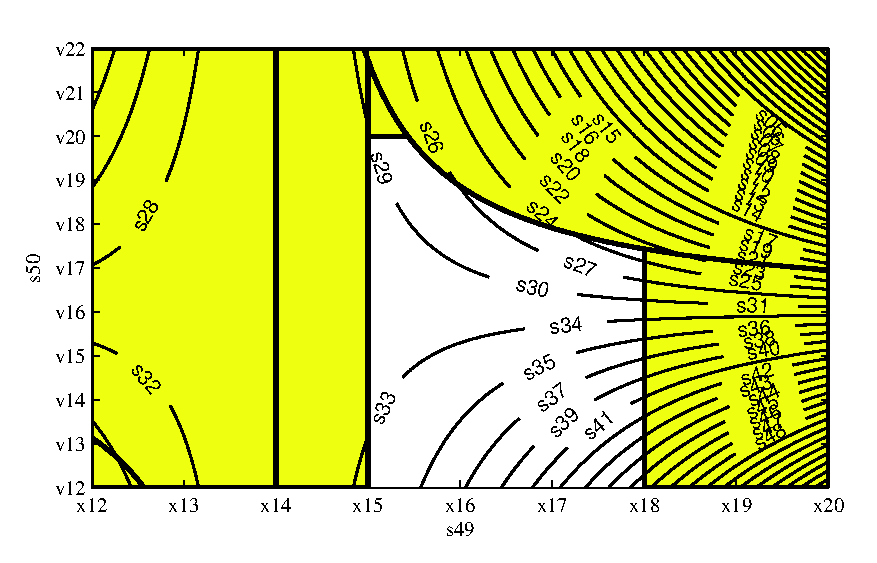
\includegraphics{./Data/Hw3/problem485.eps}}%
\end{psfrags}%
%
% End problem485.tex
\end{document}
% See http://www.mathworks.de/matlabcentral/fileexchange/loadFile.do?objectId=4638
% for recent versions of laprint.m.
%
% created by:           LaPrint version 3.16 (13.9.2004)
% created on:           28-Dec-2013 22:36:47
% eps bounding box:     15 cm x 9.4415 cm
% comment:              
%
\begin{psfrags}%
\psfragscanon%
%
% text strings:
\psfrag{s05}[][]{\color[rgb]{0,0,0}\setlength{\tabcolsep}{0pt}\begin{tabular}{c}-48787.0859\end{tabular}}%
\psfrag{s06}[][]{\color[rgb]{0,0,0}\setlength{\tabcolsep}{0pt}\begin{tabular}{c}-46015.0924\end{tabular}}%
\psfrag{s07}[][]{\color[rgb]{0,0,0}\setlength{\tabcolsep}{0pt}\begin{tabular}{c}-43243.0989\end{tabular}}%
\psfrag{s08}[][]{\color[rgb]{0,0,0}\setlength{\tabcolsep}{0pt}\begin{tabular}{c}-40471.1054\end{tabular}}%
\psfrag{s09}[][]{\color[rgb]{0,0,0}\setlength{\tabcolsep}{0pt}\begin{tabular}{c}-37699.1118\end{tabular}}%
\psfrag{s10}[][]{\color[rgb]{0,0,0}\setlength{\tabcolsep}{0pt}\begin{tabular}{c}-34927.1183\end{tabular}}%
\psfrag{s11}[][]{\color[rgb]{0,0,0}\setlength{\tabcolsep}{0pt}\begin{tabular}{c}-32155.1248\end{tabular}}%
\psfrag{s12}[][]{\color[rgb]{0,0,0}\setlength{\tabcolsep}{0pt}\begin{tabular}{c}-29383.1313\end{tabular}}%
\psfrag{s13}[][]{\color[rgb]{0,0,0}\setlength{\tabcolsep}{0pt}\begin{tabular}{c}-26611.1378\end{tabular}}%
\psfrag{s14}[][]{\color[rgb]{0,0,0}\setlength{\tabcolsep}{0pt}\begin{tabular}{c}-23839.1443\end{tabular}}%
\psfrag{s15}[][]{\color[rgb]{0,0,0}\setlength{\tabcolsep}{0pt}\begin{tabular}{c}-21067.1507\end{tabular}}%
\psfrag{s16}[][]{\color[rgb]{0,0,0}\setlength{\tabcolsep}{0pt}\begin{tabular}{c}-18295.1572\end{tabular}}%
\psfrag{s17}[][]{\color[rgb]{0,0,0}\setlength{\tabcolsep}{0pt}\begin{tabular}{c}-18295.1572\end{tabular}}%
\psfrag{s18}[][]{\color[rgb]{0,0,0}\setlength{\tabcolsep}{0pt}\begin{tabular}{c}-15523.1637\end{tabular}}%
\psfrag{s19}[][]{\color[rgb]{0,0,0}\setlength{\tabcolsep}{0pt}\begin{tabular}{c}-15523.1637\end{tabular}}%
\psfrag{s20}[][]{\color[rgb]{0,0,0}\setlength{\tabcolsep}{0pt}\begin{tabular}{c}-12751.1702\end{tabular}}%
\psfrag{s21}[][]{\color[rgb]{0,0,0}\setlength{\tabcolsep}{0pt}\begin{tabular}{c}-12751.1702\end{tabular}}%
\psfrag{s22}[][]{\color[rgb]{0,0,0}\setlength{\tabcolsep}{0pt}\begin{tabular}{c}-9979.17666\end{tabular}}%
\psfrag{s23}[][]{\color[rgb]{0,0,0}\setlength{\tabcolsep}{0pt}\begin{tabular}{c}-9979.17666\end{tabular}}%
\psfrag{s24}[][]{\color[rgb]{0,0,0}\setlength{\tabcolsep}{0pt}\begin{tabular}{c}-7207.18315\end{tabular}}%
\psfrag{s25}[][]{\color[rgb]{0,0,0}\setlength{\tabcolsep}{0pt}\begin{tabular}{c}-7207.18315\end{tabular}}%
\psfrag{s26}[][]{\color[rgb]{0,0,0}\setlength{\tabcolsep}{0pt}\begin{tabular}{c}-4435.18963\end{tabular}}%
\psfrag{s27}[][]{\color[rgb]{0,0,0}\setlength{\tabcolsep}{0pt}\begin{tabular}{c}-4435.18963\end{tabular}}%
\psfrag{s28}[][]{\color[rgb]{0,0,0}\setlength{\tabcolsep}{0pt}\begin{tabular}{c}-1663.19611\end{tabular}}%
\psfrag{s29}[][]{\color[rgb]{0,0,0}\setlength{\tabcolsep}{0pt}\begin{tabular}{c}-1663.19611\end{tabular}}%
\psfrag{s30}[][]{\color[rgb]{0,0,0}\setlength{\tabcolsep}{0pt}\begin{tabular}{c}-1663.19611\end{tabular}}%
\psfrag{s31}[][]{\color[rgb]{0,0,0}\setlength{\tabcolsep}{0pt}\begin{tabular}{c}-1663.19611\end{tabular}}%
\psfrag{s32}[][]{\color[rgb]{0,0,0}\setlength{\tabcolsep}{0pt}\begin{tabular}{c}1108.79741\end{tabular}}%
\psfrag{s33}[][]{\color[rgb]{0,0,0}\setlength{\tabcolsep}{0pt}\begin{tabular}{c}1108.79741\end{tabular}}%
\psfrag{s34}[][]{\color[rgb]{0,0,0}\setlength{\tabcolsep}{0pt}\begin{tabular}{c}1108.79741\end{tabular}}%
\psfrag{s35}[][]{\color[rgb]{0,0,0}\setlength{\tabcolsep}{0pt}\begin{tabular}{c}3880.79093\end{tabular}}%
\psfrag{s36}[][]{\color[rgb]{0,0,0}\setlength{\tabcolsep}{0pt}\begin{tabular}{c}3880.79093\end{tabular}}%
\psfrag{s37}[][]{\color[rgb]{0,0,0}\setlength{\tabcolsep}{0pt}\begin{tabular}{c}6652.78444\end{tabular}}%
\psfrag{s38}[][]{\color[rgb]{0,0,0}\setlength{\tabcolsep}{0pt}\begin{tabular}{c}6652.78444\end{tabular}}%
\psfrag{s39}[][]{\color[rgb]{0,0,0}\setlength{\tabcolsep}{0pt}\begin{tabular}{c}9424.77796\end{tabular}}%
\psfrag{s40}[][]{\color[rgb]{0,0,0}\setlength{\tabcolsep}{0pt}\begin{tabular}{c}9424.77796\end{tabular}}%
\psfrag{s41}[][]{\color[rgb]{0,0,0}\setlength{\tabcolsep}{0pt}\begin{tabular}{c}12196.7715\end{tabular}}%
\psfrag{s42}[][]{\color[rgb]{0,0,0}\setlength{\tabcolsep}{0pt}\begin{tabular}{c}14968.765\end{tabular}}%
\psfrag{s43}[][]{\color[rgb]{0,0,0}\setlength{\tabcolsep}{0pt}\begin{tabular}{c}17740.7585\end{tabular}}%
\psfrag{s44}[][]{\color[rgb]{0,0,0}\setlength{\tabcolsep}{0pt}\begin{tabular}{c}20512.752\end{tabular}}%
\psfrag{s45}[][]{\color[rgb]{0,0,0}\setlength{\tabcolsep}{0pt}\begin{tabular}{c}23284.7456\end{tabular}}%
\psfrag{s46}[][]{\color[rgb]{0,0,0}\setlength{\tabcolsep}{0pt}\begin{tabular}{c}26056.7391\end{tabular}}%
\psfrag{s47}[][]{\color[rgb]{0,0,0}\setlength{\tabcolsep}{0pt}\begin{tabular}{c}28828.7326\end{tabular}}%
\psfrag{s48}[][]{\color[rgb]{0,0,0}\setlength{\tabcolsep}{0pt}\begin{tabular}{c}31600.7261\end{tabular}}%
\psfrag{s49}[t][t]{\color[rgb]{0,0,0}\setlength{\tabcolsep}{0pt}\begin{tabular}{c}x\end{tabular}}%
\psfrag{s50}[b][b]{\color[rgb]{0,0,0}\setlength{\tabcolsep}{0pt}\begin{tabular}{c}y\end{tabular}}%

%
% xticklabels:
\psfrag{x01}[t][t]{0}%
\psfrag{x02}[t][t]{0.1}%
\psfrag{x03}[t][t]{0.2}%
\psfrag{x04}[t][t]{0.3}%
\psfrag{x05}[t][t]{0.4}%
\psfrag{x06}[t][t]{0.5}%
\psfrag{x07}[t][t]{0.6}%
\psfrag{x08}[t][t]{0.7}%
\psfrag{x09}[t][t]{0.8}%
\psfrag{x10}[t][t]{0.9}%
\psfrag{x11}[t][t]{1}%
\psfrag{x12}[t][t]{-10}%
\psfrag{x13}[t][t]{-5}%
\psfrag{x14}[t][t]{0}%
\psfrag{x15}[t][t]{5}%
\psfrag{x16}[t][t]{10}%
\psfrag{x17}[t][t]{15}%
\psfrag{x18}[t][t]{20}%
\psfrag{x19}[t][t]{25}%
\psfrag{x20}[t][t]{30}%
\psfrag{x21}[t][t]{0}%
\psfrag{x22}[t][t]{0.1}%
\psfrag{x23}[t][t]{0.2}%
\psfrag{x24}[t][t]{0.3}%
\psfrag{x25}[t][t]{0.4}%
\psfrag{x26}[t][t]{0.5}%
\psfrag{x27}[t][t]{0.6}%
\psfrag{x28}[t][t]{0.7}%
\psfrag{x29}[t][t]{0.8}%
\psfrag{x30}[t][t]{0.9}%
\psfrag{x31}[t][t]{1}%
%
% yticklabels:
\psfrag{v01}[r][r]{0}%
\psfrag{v02}[r][r]{0.1}%
\psfrag{v03}[r][r]{0.2}%
\psfrag{v04}[r][r]{0.3}%
\psfrag{v05}[r][r]{0.4}%
\psfrag{v06}[r][r]{0.5}%
\psfrag{v07}[r][r]{0.6}%
\psfrag{v08}[r][r]{0.7}%
\psfrag{v09}[r][r]{0.8}%
\psfrag{v10}[r][r]{0.9}%
\psfrag{v11}[r][r]{1}%
\psfrag{v12}[r][r]{-20}%
\psfrag{v13}[r][r]{-15}%
\psfrag{v14}[r][r]{-10}%
\psfrag{v15}[r][r]{-5}%
\psfrag{v16}[r][r]{0}%
\psfrag{v17}[r][r]{5}%
\psfrag{v18}[r][r]{10}%
\psfrag{v19}[r][r]{15}%
\psfrag{v20}[r][r]{20}%
\psfrag{v21}[r][r]{25}%
\psfrag{v22}[r][r]{30}%
\psfrag{v23}[r][r]{0}%
\psfrag{v24}[r][r]{0.1}%
\psfrag{v25}[r][r]{0.2}%
\psfrag{v26}[r][r]{0.3}%
\psfrag{v27}[r][r]{0.4}%
\psfrag{v28}[r][r]{0.5}%
\psfrag{v29}[r][r]{0.6}%
\psfrag{v30}[r][r]{0.7}%
\psfrag{v31}[r][r]{0.8}%
\psfrag{v32}[r][r]{0.9}%
\psfrag{v33}[r][r]{1}%
%
% Figure:
\resizebox{12cm}{!}{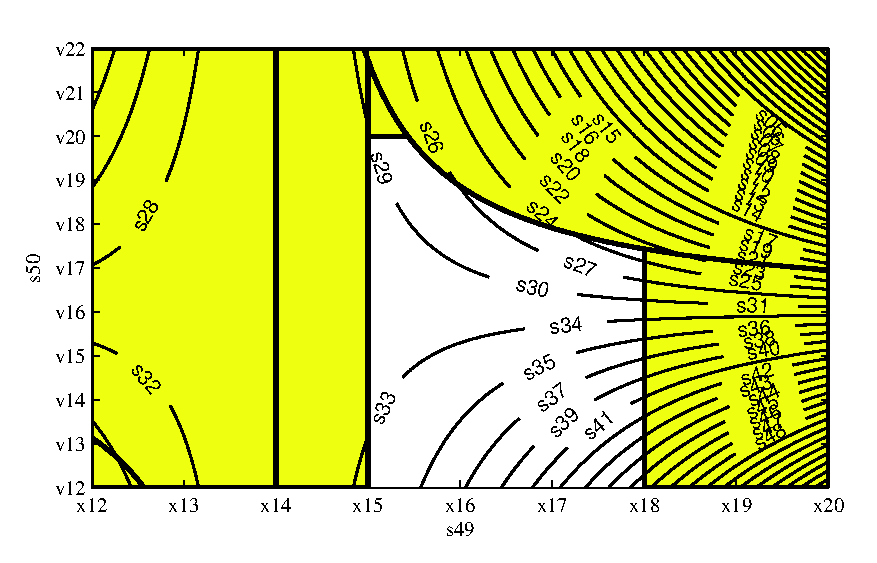
\includegraphics{./Data/Hw3/problem485.eps}}%
\end{psfrags}%
%
% End problem485.tex
\end{document}
% See http://www.mathworks.de/matlabcentral/fileexchange/loadFile.do?objectId=4638
% for recent versions of laprint.m.
%
% created by:           LaPrint version 3.16 (13.9.2004)
% created on:           28-Dec-2013 22:36:47
% eps bounding box:     15 cm x 9.4415 cm
% comment:              
%
\begin{psfrags}%
\psfragscanon%
%
% text strings:
\psfrag{s05}[][]{\color[rgb]{0,0,0}\setlength{\tabcolsep}{0pt}\begin{tabular}{c}-48787.0859\end{tabular}}%
\psfrag{s06}[][]{\color[rgb]{0,0,0}\setlength{\tabcolsep}{0pt}\begin{tabular}{c}-46015.0924\end{tabular}}%
\psfrag{s07}[][]{\color[rgb]{0,0,0}\setlength{\tabcolsep}{0pt}\begin{tabular}{c}-43243.0989\end{tabular}}%
\psfrag{s08}[][]{\color[rgb]{0,0,0}\setlength{\tabcolsep}{0pt}\begin{tabular}{c}-40471.1054\end{tabular}}%
\psfrag{s09}[][]{\color[rgb]{0,0,0}\setlength{\tabcolsep}{0pt}\begin{tabular}{c}-37699.1118\end{tabular}}%
\psfrag{s10}[][]{\color[rgb]{0,0,0}\setlength{\tabcolsep}{0pt}\begin{tabular}{c}-34927.1183\end{tabular}}%
\psfrag{s11}[][]{\color[rgb]{0,0,0}\setlength{\tabcolsep}{0pt}\begin{tabular}{c}-32155.1248\end{tabular}}%
\psfrag{s12}[][]{\color[rgb]{0,0,0}\setlength{\tabcolsep}{0pt}\begin{tabular}{c}-29383.1313\end{tabular}}%
\psfrag{s13}[][]{\color[rgb]{0,0,0}\setlength{\tabcolsep}{0pt}\begin{tabular}{c}-26611.1378\end{tabular}}%
\psfrag{s14}[][]{\color[rgb]{0,0,0}\setlength{\tabcolsep}{0pt}\begin{tabular}{c}-23839.1443\end{tabular}}%
\psfrag{s15}[][]{\color[rgb]{0,0,0}\setlength{\tabcolsep}{0pt}\begin{tabular}{c}-21067.1507\end{tabular}}%
\psfrag{s16}[][]{\color[rgb]{0,0,0}\setlength{\tabcolsep}{0pt}\begin{tabular}{c}-18295.1572\end{tabular}}%
\psfrag{s17}[][]{\color[rgb]{0,0,0}\setlength{\tabcolsep}{0pt}\begin{tabular}{c}-18295.1572\end{tabular}}%
\psfrag{s18}[][]{\color[rgb]{0,0,0}\setlength{\tabcolsep}{0pt}\begin{tabular}{c}-15523.1637\end{tabular}}%
\psfrag{s19}[][]{\color[rgb]{0,0,0}\setlength{\tabcolsep}{0pt}\begin{tabular}{c}-15523.1637\end{tabular}}%
\psfrag{s20}[][]{\color[rgb]{0,0,0}\setlength{\tabcolsep}{0pt}\begin{tabular}{c}-12751.1702\end{tabular}}%
\psfrag{s21}[][]{\color[rgb]{0,0,0}\setlength{\tabcolsep}{0pt}\begin{tabular}{c}-12751.1702\end{tabular}}%
\psfrag{s22}[][]{\color[rgb]{0,0,0}\setlength{\tabcolsep}{0pt}\begin{tabular}{c}-9979.17666\end{tabular}}%
\psfrag{s23}[][]{\color[rgb]{0,0,0}\setlength{\tabcolsep}{0pt}\begin{tabular}{c}-9979.17666\end{tabular}}%
\psfrag{s24}[][]{\color[rgb]{0,0,0}\setlength{\tabcolsep}{0pt}\begin{tabular}{c}-7207.18315\end{tabular}}%
\psfrag{s25}[][]{\color[rgb]{0,0,0}\setlength{\tabcolsep}{0pt}\begin{tabular}{c}-7207.18315\end{tabular}}%
\psfrag{s26}[][]{\color[rgb]{0,0,0}\setlength{\tabcolsep}{0pt}\begin{tabular}{c}-4435.18963\end{tabular}}%
\psfrag{s27}[][]{\color[rgb]{0,0,0}\setlength{\tabcolsep}{0pt}\begin{tabular}{c}-4435.18963\end{tabular}}%
\psfrag{s28}[][]{\color[rgb]{0,0,0}\setlength{\tabcolsep}{0pt}\begin{tabular}{c}-1663.19611\end{tabular}}%
\psfrag{s29}[][]{\color[rgb]{0,0,0}\setlength{\tabcolsep}{0pt}\begin{tabular}{c}-1663.19611\end{tabular}}%
\psfrag{s30}[][]{\color[rgb]{0,0,0}\setlength{\tabcolsep}{0pt}\begin{tabular}{c}-1663.19611\end{tabular}}%
\psfrag{s31}[][]{\color[rgb]{0,0,0}\setlength{\tabcolsep}{0pt}\begin{tabular}{c}-1663.19611\end{tabular}}%
\psfrag{s32}[][]{\color[rgb]{0,0,0}\setlength{\tabcolsep}{0pt}\begin{tabular}{c}1108.79741\end{tabular}}%
\psfrag{s33}[][]{\color[rgb]{0,0,0}\setlength{\tabcolsep}{0pt}\begin{tabular}{c}1108.79741\end{tabular}}%
\psfrag{s34}[][]{\color[rgb]{0,0,0}\setlength{\tabcolsep}{0pt}\begin{tabular}{c}1108.79741\end{tabular}}%
\psfrag{s35}[][]{\color[rgb]{0,0,0}\setlength{\tabcolsep}{0pt}\begin{tabular}{c}3880.79093\end{tabular}}%
\psfrag{s36}[][]{\color[rgb]{0,0,0}\setlength{\tabcolsep}{0pt}\begin{tabular}{c}3880.79093\end{tabular}}%
\psfrag{s37}[][]{\color[rgb]{0,0,0}\setlength{\tabcolsep}{0pt}\begin{tabular}{c}6652.78444\end{tabular}}%
\psfrag{s38}[][]{\color[rgb]{0,0,0}\setlength{\tabcolsep}{0pt}\begin{tabular}{c}6652.78444\end{tabular}}%
\psfrag{s39}[][]{\color[rgb]{0,0,0}\setlength{\tabcolsep}{0pt}\begin{tabular}{c}9424.77796\end{tabular}}%
\psfrag{s40}[][]{\color[rgb]{0,0,0}\setlength{\tabcolsep}{0pt}\begin{tabular}{c}9424.77796\end{tabular}}%
\psfrag{s41}[][]{\color[rgb]{0,0,0}\setlength{\tabcolsep}{0pt}\begin{tabular}{c}12196.7715\end{tabular}}%
\psfrag{s42}[][]{\color[rgb]{0,0,0}\setlength{\tabcolsep}{0pt}\begin{tabular}{c}14968.765\end{tabular}}%
\psfrag{s43}[][]{\color[rgb]{0,0,0}\setlength{\tabcolsep}{0pt}\begin{tabular}{c}17740.7585\end{tabular}}%
\psfrag{s44}[][]{\color[rgb]{0,0,0}\setlength{\tabcolsep}{0pt}\begin{tabular}{c}20512.752\end{tabular}}%
\psfrag{s45}[][]{\color[rgb]{0,0,0}\setlength{\tabcolsep}{0pt}\begin{tabular}{c}23284.7456\end{tabular}}%
\psfrag{s46}[][]{\color[rgb]{0,0,0}\setlength{\tabcolsep}{0pt}\begin{tabular}{c}26056.7391\end{tabular}}%
\psfrag{s47}[][]{\color[rgb]{0,0,0}\setlength{\tabcolsep}{0pt}\begin{tabular}{c}28828.7326\end{tabular}}%
\psfrag{s48}[][]{\color[rgb]{0,0,0}\setlength{\tabcolsep}{0pt}\begin{tabular}{c}31600.7261\end{tabular}}%
\psfrag{s49}[t][t]{\color[rgb]{0,0,0}\setlength{\tabcolsep}{0pt}\begin{tabular}{c}x\end{tabular}}%
\psfrag{s50}[b][b]{\color[rgb]{0,0,0}\setlength{\tabcolsep}{0pt}\begin{tabular}{c}y\end{tabular}}%

%
% xticklabels:
\psfrag{x01}[t][t]{0}%
\psfrag{x02}[t][t]{0.1}%
\psfrag{x03}[t][t]{0.2}%
\psfrag{x04}[t][t]{0.3}%
\psfrag{x05}[t][t]{0.4}%
\psfrag{x06}[t][t]{0.5}%
\psfrag{x07}[t][t]{0.6}%
\psfrag{x08}[t][t]{0.7}%
\psfrag{x09}[t][t]{0.8}%
\psfrag{x10}[t][t]{0.9}%
\psfrag{x11}[t][t]{1}%
\psfrag{x12}[t][t]{-10}%
\psfrag{x13}[t][t]{-5}%
\psfrag{x14}[t][t]{0}%
\psfrag{x15}[t][t]{5}%
\psfrag{x16}[t][t]{10}%
\psfrag{x17}[t][t]{15}%
\psfrag{x18}[t][t]{20}%
\psfrag{x19}[t][t]{25}%
\psfrag{x20}[t][t]{30}%
\psfrag{x21}[t][t]{0}%
\psfrag{x22}[t][t]{0.1}%
\psfrag{x23}[t][t]{0.2}%
\psfrag{x24}[t][t]{0.3}%
\psfrag{x25}[t][t]{0.4}%
\psfrag{x26}[t][t]{0.5}%
\psfrag{x27}[t][t]{0.6}%
\psfrag{x28}[t][t]{0.7}%
\psfrag{x29}[t][t]{0.8}%
\psfrag{x30}[t][t]{0.9}%
\psfrag{x31}[t][t]{1}%
%
% yticklabels:
\psfrag{v01}[r][r]{0}%
\psfrag{v02}[r][r]{0.1}%
\psfrag{v03}[r][r]{0.2}%
\psfrag{v04}[r][r]{0.3}%
\psfrag{v05}[r][r]{0.4}%
\psfrag{v06}[r][r]{0.5}%
\psfrag{v07}[r][r]{0.6}%
\psfrag{v08}[r][r]{0.7}%
\psfrag{v09}[r][r]{0.8}%
\psfrag{v10}[r][r]{0.9}%
\psfrag{v11}[r][r]{1}%
\psfrag{v12}[r][r]{-20}%
\psfrag{v13}[r][r]{-15}%
\psfrag{v14}[r][r]{-10}%
\psfrag{v15}[r][r]{-5}%
\psfrag{v16}[r][r]{0}%
\psfrag{v17}[r][r]{5}%
\psfrag{v18}[r][r]{10}%
\psfrag{v19}[r][r]{15}%
\psfrag{v20}[r][r]{20}%
\psfrag{v21}[r][r]{25}%
\psfrag{v22}[r][r]{30}%
\psfrag{v23}[r][r]{0}%
\psfrag{v24}[r][r]{0.1}%
\psfrag{v25}[r][r]{0.2}%
\psfrag{v26}[r][r]{0.3}%
\psfrag{v27}[r][r]{0.4}%
\psfrag{v28}[r][r]{0.5}%
\psfrag{v29}[r][r]{0.6}%
\psfrag{v30}[r][r]{0.7}%
\psfrag{v31}[r][r]{0.8}%
\psfrag{v32}[r][r]{0.9}%
\psfrag{v33}[r][r]{1}%
%
% Figure:
\resizebox{12cm}{!}{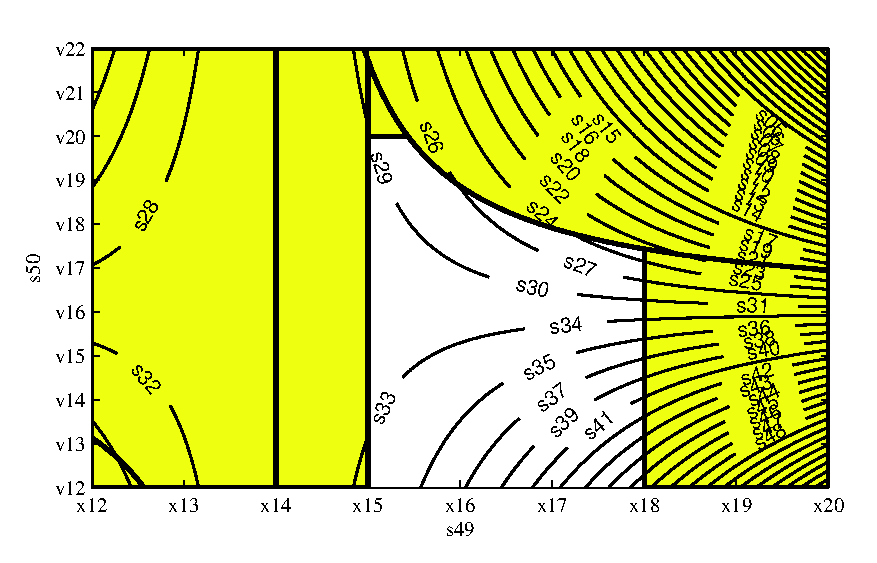
\includegraphics{./Data/Hw3/problem485.eps}}%
\end{psfrags}%
%
% End problem485.tex

\caption{Plot of the cost function and constraints of problem 4.85.}
\label{fig:problem485}
\end{figure}
\\
From \cref{fig:problem485}, it is seen that increasing value of the both $x$ and $y$ decreases the value of the cost function. Within the feasible region, the minimum value of the function is found to be $9000$ at $\left(x^*,y^*\right)=\left(20\, ,\,  7.162\right)$.
\\~
\\
For the verification of KKT conditions of the problem we should write Lagrangian which is given by the following equation
\begin{eqnarray*}
L &=&f\left(\mathbf x\right) + \mathbf{v}^T\mathbf{h}+\mathbf{u}^T\left(\mathbf{g}+\mathbf{s}^2\right)
\end{eqnarray*}
Thus, Lagrangian of the problem is 
\begin{eqnarray*}
L \left(x,y\right) &=&-\pi x^2 y+u_1\left(x-20+s_1^2\right)+u_2\left(y-20+s_2^2\right)+\\
&& u_3\left(5-x+s_3^2\right)+u_4\left(-x+s_4^2\right)+u_5\left(2\pi x y -900+s_5^2\right)
\end{eqnarray*}
The stationary point conditions are found as
\begin{eqnarray*}
\frac{\partial L}{\partial x}&=& 0 \; ; \; -2 \pi x y +u_1-u_3-u_4+2\pi u_5 y=0
\\ \frac{\partial L}{\partial y}&=& 0 \; ; \; - \pi x^2 y +2\pi u_5x=0
\\
\frac{\partial L}{\partial u_1}&=& 0 \; ; \; x-20+s_1^2=0
\\
\frac{\partial L}{\partial u_2}&=& 0 \; ; \; y-20+s_2^2=0
\\
\frac{\partial L}{\partial u_3}&=& 0 \; ; \; 5-x+s_3^2=0
\\
\frac{\partial L}{\partial u_4}&=& 0 \; ; \; -x+s_4^2=0
\\
\frac{\partial L}{\partial u_5}&=& 0 \; ; \; -2 \pi x y -900+s_5^2=0
\\
\frac{\partial L}{\partial s_1}&=& 0 \; ; \; 2 u_1 s_1=0
\\
\frac{\partial L}{\partial s_2}&=& 0 \; ; \; 2 u_2 s_2=0
\\
\frac{\partial L}{\partial s_3}&=& 0 \; ; \; 2 u_3 s_3=0
\\
\frac{\partial L}{\partial s_4}&=& 0 \; ; \; 2 u_4 s_4=0
\\
\frac{\partial L}{\partial s_5}&=& 0 \; ; \; 2 u_5 s_5=0
\end{eqnarray*}
Evaluating the conditions at the graphically found solution point $\left(x^*,y^*\right)=\left(20\, ,\,  7.162\right)$ , the unknowns of the problem are found as
\begin{eqnarray*}
\begin{array}{lc}
 x=20\;,\;y=7.16\;,\;s_1=0\;,\;u_2=0\;,\;u_3=0\;,\; u_4=0\;,\; s_5=0\;,&\\ u_5=10\;,\;u_1=449.876\;,\;s_2=3.583\;,\; s_3=3.873\;,\; s_4=4.472\;&
 \end{array}
\end{eqnarray*}
Slack variables of constraints of $g_1$ and $g_5$ is found to be zero at the solution point, thus, they are both active.
\subsection*{Problem 4.101}
Solve the following problem graphically, verify the KKT neccessary conditions for the solution points and study the effect on the cost function of changing the boundary of the equality constraint by one unit.\\ 
~
\\
Minimize:
\begin{eqnarray*}
f\left(\mathbf x\right) &=& 9 x_1^2+18x_1 x_2+13x_2^2-4
\end{eqnarray*} 
Subject to:
\begin{eqnarray*}
x_1^2+x_2^2+2x_1&=& 16
\end{eqnarray*} 
\subsubsection*{Solution}
Plots of the cost function and equality constraints of the problem is given in \cref{fig:problem4101}.
\begin{figure}[ht!]
% This file is generated by the MATLAB m-file laprint.m. It can be included
% into LaTeX documents using the packages graphicx, color and psfrag.
% It is accompanied by a postscript file. A sample LaTeX file is:
%    \documentclass{article}\usepackage{graphicx,color,psfrag}
%    \begin{document}% This file is generated by the MATLAB m-file laprint.m. It can be included
% into LaTeX documents using the packages graphicx, color and psfrag.
% It is accompanied by a postscript file. A sample LaTeX file is:
%    \documentclass{article}\usepackage{graphicx,color,psfrag}
%    \begin{document}% This file is generated by the MATLAB m-file laprint.m. It can be included
% into LaTeX documents using the packages graphicx, color and psfrag.
% It is accompanied by a postscript file. A sample LaTeX file is:
%    \documentclass{article}\usepackage{graphicx,color,psfrag}
%    \begin{document}\input{problem4101}\end{document}
% See http://www.mathworks.de/matlabcentral/fileexchange/loadFile.do?objectId=4638
% for recent versions of laprint.m.
%
% created by:           LaPrint version 3.16 (13.9.2004)
% created on:           28-Dec-2013 23:06:44
% eps bounding box:     15 cm x 9.4415 cm
% comment:              
%
\begin{psfrags}%
\psfragscanon%
%
% text strings:
\psfrag{s01}[][]{\fontsize{10}{15}\fontseries{m}\mathversion{normal}\fontshape{n}\selectfont \color[rgb]{0,0,0}\setlength{\tabcolsep}{0pt}\begin{tabular}{c}0\end{tabular}}%
\psfrag{s02}[][]{\fontsize{10}{15}\fontseries{m}\mathversion{normal}\fontshape{n}\selectfont \color[rgb]{0,0,0}\setlength{\tabcolsep}{0pt}\begin{tabular}{c}0\end{tabular}}%
\psfrag{s03}[][]{\fontsize{10}{15}\fontseries{m}\mathversion{normal}\fontshape{n}\selectfont \color[rgb]{0,0,0}\setlength{\tabcolsep}{0pt}\begin{tabular}{c}0\end{tabular}}%
\psfrag{s04}[][]{\fontsize{10}{15}\fontseries{m}\mathversion{normal}\fontshape{n}\selectfont \color[rgb]{0,0,0}\setlength{\tabcolsep}{0pt}\begin{tabular}{c}10\end{tabular}}%
\psfrag{s05}[][]{\fontsize{10}{15}\fontseries{m}\mathversion{normal}\fontshape{n}\selectfont \color[rgb]{0,0,0}\setlength{\tabcolsep}{0pt}\begin{tabular}{c}10\end{tabular}}%
\psfrag{s06}[][]{\fontsize{10}{15}\fontseries{m}\mathversion{normal}\fontshape{n}\selectfont \color[rgb]{0,0,0}\setlength{\tabcolsep}{0pt}\begin{tabular}{c}10\end{tabular}}%
\psfrag{s07}[][]{\fontsize{10}{15}\fontseries{m}\mathversion{normal}\fontshape{n}\selectfont \color[rgb]{0,0,0}\setlength{\tabcolsep}{0pt}\begin{tabular}{c}10\end{tabular}}%
\psfrag{s08}[][]{\fontsize{10}{15}\fontseries{m}\mathversion{normal}\fontshape{n}\selectfont \color[rgb]{0,0,0}\setlength{\tabcolsep}{0pt}\begin{tabular}{c}10\end{tabular}}%
\psfrag{s09}[][]{\fontsize{10}{15}\fontseries{m}\mathversion{normal}\fontshape{n}\selectfont \color[rgb]{0,0,0}\setlength{\tabcolsep}{0pt}\begin{tabular}{c}20\end{tabular}}%
\psfrag{s10}[][]{\fontsize{10}{15}\fontseries{m}\mathversion{normal}\fontshape{n}\selectfont \color[rgb]{0,0,0}\setlength{\tabcolsep}{0pt}\begin{tabular}{c}20\end{tabular}}%
\psfrag{s11}[][]{\fontsize{10}{15}\fontseries{m}\mathversion{normal}\fontshape{n}\selectfont \color[rgb]{0,0,0}\setlength{\tabcolsep}{0pt}\begin{tabular}{c}20\end{tabular}}%
\psfrag{s12}[][]{\fontsize{10}{15}\fontseries{m}\mathversion{normal}\fontshape{n}\selectfont \color[rgb]{0,0,0}\setlength{\tabcolsep}{0pt}\begin{tabular}{c}20\end{tabular}}%
\psfrag{s13}[][]{\fontsize{10}{15}\fontseries{m}\mathversion{normal}\fontshape{n}\selectfont \color[rgb]{0,0,0}\setlength{\tabcolsep}{0pt}\begin{tabular}{c}20\end{tabular}}%
\psfrag{s14}[][]{\fontsize{10}{15}\fontseries{m}\mathversion{normal}\fontshape{n}\selectfont \color[rgb]{0,0,0}\setlength{\tabcolsep}{0pt}\begin{tabular}{c}20\end{tabular}}%
\psfrag{s15}[][]{\fontsize{10}{15}\fontseries{m}\mathversion{normal}\fontshape{n}\selectfont \color[rgb]{0,0,0}\setlength{\tabcolsep}{0pt}\begin{tabular}{c}30\end{tabular}}%
\psfrag{s16}[][]{\fontsize{10}{15}\fontseries{m}\mathversion{normal}\fontshape{n}\selectfont \color[rgb]{0,0,0}\setlength{\tabcolsep}{0pt}\begin{tabular}{c}30\end{tabular}}%
\psfrag{s17}[][]{\fontsize{10}{15}\fontseries{m}\mathversion{normal}\fontshape{n}\selectfont \color[rgb]{0,0,0}\setlength{\tabcolsep}{0pt}\begin{tabular}{c}30\end{tabular}}%
\psfrag{s18}[][]{\fontsize{10}{15}\fontseries{m}\mathversion{normal}\fontshape{n}\selectfont \color[rgb]{0,0,0}\setlength{\tabcolsep}{0pt}\begin{tabular}{c}30\end{tabular}}%
\psfrag{s19}[][]{\fontsize{10}{15}\fontseries{m}\mathversion{normal}\fontshape{n}\selectfont \color[rgb]{0,0,0}\setlength{\tabcolsep}{0pt}\begin{tabular}{c}30\end{tabular}}%
\psfrag{s20}[][]{\fontsize{10}{15}\fontseries{m}\mathversion{normal}\fontshape{n}\selectfont \color[rgb]{0,0,0}\setlength{\tabcolsep}{0pt}\begin{tabular}{c}30\end{tabular}}%
\psfrag{s21}[][]{\fontsize{10}{15}\fontseries{m}\mathversion{normal}\fontshape{n}\selectfont \color[rgb]{0,0,0}\setlength{\tabcolsep}{0pt}\begin{tabular}{c}40\end{tabular}}%
\psfrag{s22}[][]{\fontsize{10}{15}\fontseries{m}\mathversion{normal}\fontshape{n}\selectfont \color[rgb]{0,0,0}\setlength{\tabcolsep}{0pt}\begin{tabular}{c}40\end{tabular}}%
\psfrag{s23}[][]{\fontsize{10}{15}\fontseries{m}\mathversion{normal}\fontshape{n}\selectfont \color[rgb]{0,0,0}\setlength{\tabcolsep}{0pt}\begin{tabular}{c}40\end{tabular}}%
\psfrag{s24}[][]{\fontsize{10}{15}\fontseries{m}\mathversion{normal}\fontshape{n}\selectfont \color[rgb]{0,0,0}\setlength{\tabcolsep}{0pt}\begin{tabular}{c}40\end{tabular}}%
\psfrag{s25}[][]{\fontsize{10}{15}\fontseries{m}\mathversion{normal}\fontshape{n}\selectfont \color[rgb]{0,0,0}\setlength{\tabcolsep}{0pt}\begin{tabular}{c}40\end{tabular}}%
\psfrag{s26}[][]{\fontsize{10}{15}\fontseries{m}\mathversion{normal}\fontshape{n}\selectfont \color[rgb]{0,0,0}\setlength{\tabcolsep}{0pt}\begin{tabular}{c}40\end{tabular}}%
\psfrag{s27}[][]{\fontsize{10}{15}\fontseries{m}\mathversion{normal}\fontshape{n}\selectfont \color[rgb]{0,0,0}\setlength{\tabcolsep}{0pt}\begin{tabular}{c}40\end{tabular}}%
\psfrag{s28}[][]{\fontsize{10}{15}\fontseries{m}\mathversion{normal}\fontshape{n}\selectfont \color[rgb]{0,0,0}\setlength{\tabcolsep}{0pt}\begin{tabular}{c}50\end{tabular}}%
\psfrag{s29}[][]{\fontsize{10}{15}\fontseries{m}\mathversion{normal}\fontshape{n}\selectfont \color[rgb]{0,0,0}\setlength{\tabcolsep}{0pt}\begin{tabular}{c}50\end{tabular}}%
\psfrag{s30}[][]{\fontsize{10}{15}\fontseries{m}\mathversion{normal}\fontshape{n}\selectfont \color[rgb]{0,0,0}\setlength{\tabcolsep}{0pt}\begin{tabular}{c}50\end{tabular}}%
\psfrag{s31}[][]{\fontsize{10}{15}\fontseries{m}\mathversion{normal}\fontshape{n}\selectfont \color[rgb]{0,0,0}\setlength{\tabcolsep}{0pt}\begin{tabular}{c}50\end{tabular}}%
\psfrag{s32}[][]{\fontsize{10}{15}\fontseries{m}\mathversion{normal}\fontshape{n}\selectfont \color[rgb]{0,0,0}\setlength{\tabcolsep}{0pt}\begin{tabular}{c}50\end{tabular}}%
\psfrag{s33}[][]{\fontsize{10}{15}\fontseries{m}\mathversion{normal}\fontshape{n}\selectfont \color[rgb]{0,0,0}\setlength{\tabcolsep}{0pt}\begin{tabular}{c}50\end{tabular}}%
\psfrag{s34}[][]{\fontsize{10}{15}\fontseries{m}\mathversion{normal}\fontshape{n}\selectfont \color[rgb]{0,0,0}\setlength{\tabcolsep}{0pt}\begin{tabular}{c}50\end{tabular}}%
\psfrag{s35}[][]{\fontsize{10}{15}\fontseries{m}\mathversion{normal}\fontshape{n}\selectfont \color[rgb]{0,0,0}\setlength{\tabcolsep}{0pt}\begin{tabular}{c}60\end{tabular}}%
\psfrag{s36}[][]{\fontsize{10}{15}\fontseries{m}\mathversion{normal}\fontshape{n}\selectfont \color[rgb]{0,0,0}\setlength{\tabcolsep}{0pt}\begin{tabular}{c}60\end{tabular}}%
\psfrag{s37}[][]{\fontsize{10}{15}\fontseries{m}\mathversion{normal}\fontshape{n}\selectfont \color[rgb]{0,0,0}\setlength{\tabcolsep}{0pt}\begin{tabular}{c}60\end{tabular}}%
\psfrag{s38}[][]{\fontsize{10}{15}\fontseries{m}\mathversion{normal}\fontshape{n}\selectfont \color[rgb]{0,0,0}\setlength{\tabcolsep}{0pt}\begin{tabular}{c}60\end{tabular}}%
\psfrag{s39}[][]{\fontsize{10}{15}\fontseries{m}\mathversion{normal}\fontshape{n}\selectfont \color[rgb]{0,0,0}\setlength{\tabcolsep}{0pt}\begin{tabular}{c}60\end{tabular}}%
\psfrag{s40}[][]{\fontsize{10}{15}\fontseries{m}\mathversion{normal}\fontshape{n}\selectfont \color[rgb]{0,0,0}\setlength{\tabcolsep}{0pt}\begin{tabular}{c}60\end{tabular}}%
\psfrag{s41}[][]{\fontsize{10}{15}\fontseries{m}\mathversion{normal}\fontshape{n}\selectfont \color[rgb]{0,0,0}\setlength{\tabcolsep}{0pt}\begin{tabular}{c}60\end{tabular}}%
\psfrag{s42}[][]{\fontsize{10}{15}\fontseries{m}\mathversion{normal}\fontshape{n}\selectfont \color[rgb]{0,0,0}\setlength{\tabcolsep}{0pt}\begin{tabular}{c}60\end{tabular}}%
\psfrag{s43}[][]{\fontsize{10}{15}\fontseries{m}\mathversion{normal}\fontshape{n}\selectfont \color[rgb]{0,0,0}\setlength{\tabcolsep}{0pt}\begin{tabular}{c}70\end{tabular}}%
\psfrag{s44}[][]{\fontsize{10}{15}\fontseries{m}\mathversion{normal}\fontshape{n}\selectfont \color[rgb]{0,0,0}\setlength{\tabcolsep}{0pt}\begin{tabular}{c}70\end{tabular}}%
\psfrag{s45}[][]{\fontsize{10}{15}\fontseries{m}\mathversion{normal}\fontshape{n}\selectfont \color[rgb]{0,0,0}\setlength{\tabcolsep}{0pt}\begin{tabular}{c}70\end{tabular}}%
\psfrag{s46}[][]{\fontsize{10}{15}\fontseries{m}\mathversion{normal}\fontshape{n}\selectfont \color[rgb]{0,0,0}\setlength{\tabcolsep}{0pt}\begin{tabular}{c}70\end{tabular}}%
\psfrag{s47}[][]{\fontsize{10}{15}\fontseries{m}\mathversion{normal}\fontshape{n}\selectfont \color[rgb]{0,0,0}\setlength{\tabcolsep}{0pt}\begin{tabular}{c}70\end{tabular}}%
\psfrag{s48}[][]{\fontsize{10}{15}\fontseries{m}\mathversion{normal}\fontshape{n}\selectfont \color[rgb]{0,0,0}\setlength{\tabcolsep}{0pt}\begin{tabular}{c}70\end{tabular}}%
\psfrag{s49}[][]{\fontsize{10}{15}\fontseries{m}\mathversion{normal}\fontshape{n}\selectfont \color[rgb]{0,0,0}\setlength{\tabcolsep}{0pt}\begin{tabular}{c}70\end{tabular}}%
\psfrag{s50}[][]{\fontsize{10}{15}\fontseries{m}\mathversion{normal}\fontshape{n}\selectfont \color[rgb]{0,0,0}\setlength{\tabcolsep}{0pt}\begin{tabular}{c}15.24\end{tabular}}%
\psfrag{s51}[][]{\fontsize{10}{15}\fontseries{m}\mathversion{normal}\fontshape{n}\selectfont \color[rgb]{0,0,0}\setlength{\tabcolsep}{0pt}\begin{tabular}{c}15.24\end{tabular}}%
\psfrag{s52}[][]{\fontsize{10}{15}\fontseries{m}\mathversion{normal}\fontshape{n}\selectfont \color[rgb]{0,0,0}\setlength{\tabcolsep}{0pt}\begin{tabular}{c}15.24\end{tabular}}%
\psfrag{s53}[][]{\fontsize{10}{15}\fontseries{m}\mathversion{normal}\fontshape{n}\selectfont \color[rgb]{0,0,0}\setlength{\tabcolsep}{0pt}\begin{tabular}{c}15.24\end{tabular}}%
\psfrag{s54}[][]{\fontsize{10}{15}\fontseries{m}\mathversion{normal}\fontshape{n}\selectfont \color[rgb]{0,0,0}\setlength{\tabcolsep}{0pt}\begin{tabular}{c}15.24\end{tabular}}%
\psfrag{s55}[t][t]{\fontsize{10}{15}\fontseries{m}\mathversion{normal}\fontshape{n}\selectfont \color[rgb]{0,0,0}\setlength{\tabcolsep}{0pt}\begin{tabular}{c}$x_1$\end{tabular}}%
\psfrag{s56}[b][b]{\fontsize{10}{15}\fontseries{m}\mathversion{normal}\fontshape{n}\selectfont \color[rgb]{0,0,0}\setlength{\tabcolsep}{0pt}\begin{tabular}{c}$x_2$\end{tabular}}%
\psfrag{s63}[rb][rb]{\fontsize{16}{24}\fontseries{bx}\mathversion{bold}\fontshape{n}\selectfont \color[rgb]{0,0,0}\setlength{\tabcolsep}{0pt}\begin{tabular}{r}$F_{min}$\end{tabular}}%
%
% axes font properties:
\fontsize{10}{15}\fontseries{m}\mathversion{normal}%
\fontshape{n}\selectfont%
%
% xticklabels:
\psfrag{x01}[t][t]{0}%
\psfrag{x02}[t][t]{0.1}%
\psfrag{x03}[t][t]{0.2}%
\psfrag{x04}[t][t]{0.3}%
\psfrag{x05}[t][t]{0.4}%
\psfrag{x06}[t][t]{0.5}%
\psfrag{x07}[t][t]{0.6}%
\psfrag{x08}[t][t]{0.7}%
\psfrag{x09}[t][t]{0.8}%
\psfrag{x10}[t][t]{0.9}%
\psfrag{x11}[t][t]{1}%
\psfrag{x12}[t][t]{-5}%
\psfrag{x13}[t][t]{-4}%
\psfrag{x14}[t][t]{-3}%
\psfrag{x15}[t][t]{-2}%
\psfrag{x16}[t][t]{-1}%
\psfrag{x17}[t][t]{0}%
\psfrag{x18}[t][t]{1}%
\psfrag{x19}[t][t]{2}%
\psfrag{x20}[t][t]{3}%
%
% yticklabels:
\psfrag{v01}[r][r]{0}%
\psfrag{v02}[r][r]{0.1}%
\psfrag{v03}[r][r]{0.2}%
\psfrag{v04}[r][r]{0.3}%
\psfrag{v05}[r][r]{0.4}%
\psfrag{v06}[r][r]{0.5}%
\psfrag{v07}[r][r]{0.6}%
\psfrag{v08}[r][r]{0.7}%
\psfrag{v09}[r][r]{0.8}%
\psfrag{v10}[r][r]{0.9}%
\psfrag{v11}[r][r]{1}%
\psfrag{v12}[r][r]{-4}%
\psfrag{v13}[r][r]{-3}%
\psfrag{v14}[r][r]{-2}%
\psfrag{v15}[r][r]{-1}%
\psfrag{v16}[r][r]{0}%
\psfrag{v17}[r][r]{1}%
\psfrag{v18}[r][r]{2}%
\psfrag{v19}[r][r]{3}%
\psfrag{v20}[r][r]{4}%
%
% Figure:
\resizebox{12cm}{!}{\includegraphics{./Data/Hw3/problem4101.eps}}%
\end{psfrags}%
%
% End problem4101.tex
\end{document}
% See http://www.mathworks.de/matlabcentral/fileexchange/loadFile.do?objectId=4638
% for recent versions of laprint.m.
%
% created by:           LaPrint version 3.16 (13.9.2004)
% created on:           28-Dec-2013 23:06:44
% eps bounding box:     15 cm x 9.4415 cm
% comment:              
%
\begin{psfrags}%
\psfragscanon%
%
% text strings:
\psfrag{s01}[][]{\fontsize{10}{15}\fontseries{m}\mathversion{normal}\fontshape{n}\selectfont \color[rgb]{0,0,0}\setlength{\tabcolsep}{0pt}\begin{tabular}{c}0\end{tabular}}%
\psfrag{s02}[][]{\fontsize{10}{15}\fontseries{m}\mathversion{normal}\fontshape{n}\selectfont \color[rgb]{0,0,0}\setlength{\tabcolsep}{0pt}\begin{tabular}{c}0\end{tabular}}%
\psfrag{s03}[][]{\fontsize{10}{15}\fontseries{m}\mathversion{normal}\fontshape{n}\selectfont \color[rgb]{0,0,0}\setlength{\tabcolsep}{0pt}\begin{tabular}{c}0\end{tabular}}%
\psfrag{s04}[][]{\fontsize{10}{15}\fontseries{m}\mathversion{normal}\fontshape{n}\selectfont \color[rgb]{0,0,0}\setlength{\tabcolsep}{0pt}\begin{tabular}{c}10\end{tabular}}%
\psfrag{s05}[][]{\fontsize{10}{15}\fontseries{m}\mathversion{normal}\fontshape{n}\selectfont \color[rgb]{0,0,0}\setlength{\tabcolsep}{0pt}\begin{tabular}{c}10\end{tabular}}%
\psfrag{s06}[][]{\fontsize{10}{15}\fontseries{m}\mathversion{normal}\fontshape{n}\selectfont \color[rgb]{0,0,0}\setlength{\tabcolsep}{0pt}\begin{tabular}{c}10\end{tabular}}%
\psfrag{s07}[][]{\fontsize{10}{15}\fontseries{m}\mathversion{normal}\fontshape{n}\selectfont \color[rgb]{0,0,0}\setlength{\tabcolsep}{0pt}\begin{tabular}{c}10\end{tabular}}%
\psfrag{s08}[][]{\fontsize{10}{15}\fontseries{m}\mathversion{normal}\fontshape{n}\selectfont \color[rgb]{0,0,0}\setlength{\tabcolsep}{0pt}\begin{tabular}{c}10\end{tabular}}%
\psfrag{s09}[][]{\fontsize{10}{15}\fontseries{m}\mathversion{normal}\fontshape{n}\selectfont \color[rgb]{0,0,0}\setlength{\tabcolsep}{0pt}\begin{tabular}{c}20\end{tabular}}%
\psfrag{s10}[][]{\fontsize{10}{15}\fontseries{m}\mathversion{normal}\fontshape{n}\selectfont \color[rgb]{0,0,0}\setlength{\tabcolsep}{0pt}\begin{tabular}{c}20\end{tabular}}%
\psfrag{s11}[][]{\fontsize{10}{15}\fontseries{m}\mathversion{normal}\fontshape{n}\selectfont \color[rgb]{0,0,0}\setlength{\tabcolsep}{0pt}\begin{tabular}{c}20\end{tabular}}%
\psfrag{s12}[][]{\fontsize{10}{15}\fontseries{m}\mathversion{normal}\fontshape{n}\selectfont \color[rgb]{0,0,0}\setlength{\tabcolsep}{0pt}\begin{tabular}{c}20\end{tabular}}%
\psfrag{s13}[][]{\fontsize{10}{15}\fontseries{m}\mathversion{normal}\fontshape{n}\selectfont \color[rgb]{0,0,0}\setlength{\tabcolsep}{0pt}\begin{tabular}{c}20\end{tabular}}%
\psfrag{s14}[][]{\fontsize{10}{15}\fontseries{m}\mathversion{normal}\fontshape{n}\selectfont \color[rgb]{0,0,0}\setlength{\tabcolsep}{0pt}\begin{tabular}{c}20\end{tabular}}%
\psfrag{s15}[][]{\fontsize{10}{15}\fontseries{m}\mathversion{normal}\fontshape{n}\selectfont \color[rgb]{0,0,0}\setlength{\tabcolsep}{0pt}\begin{tabular}{c}30\end{tabular}}%
\psfrag{s16}[][]{\fontsize{10}{15}\fontseries{m}\mathversion{normal}\fontshape{n}\selectfont \color[rgb]{0,0,0}\setlength{\tabcolsep}{0pt}\begin{tabular}{c}30\end{tabular}}%
\psfrag{s17}[][]{\fontsize{10}{15}\fontseries{m}\mathversion{normal}\fontshape{n}\selectfont \color[rgb]{0,0,0}\setlength{\tabcolsep}{0pt}\begin{tabular}{c}30\end{tabular}}%
\psfrag{s18}[][]{\fontsize{10}{15}\fontseries{m}\mathversion{normal}\fontshape{n}\selectfont \color[rgb]{0,0,0}\setlength{\tabcolsep}{0pt}\begin{tabular}{c}30\end{tabular}}%
\psfrag{s19}[][]{\fontsize{10}{15}\fontseries{m}\mathversion{normal}\fontshape{n}\selectfont \color[rgb]{0,0,0}\setlength{\tabcolsep}{0pt}\begin{tabular}{c}30\end{tabular}}%
\psfrag{s20}[][]{\fontsize{10}{15}\fontseries{m}\mathversion{normal}\fontshape{n}\selectfont \color[rgb]{0,0,0}\setlength{\tabcolsep}{0pt}\begin{tabular}{c}30\end{tabular}}%
\psfrag{s21}[][]{\fontsize{10}{15}\fontseries{m}\mathversion{normal}\fontshape{n}\selectfont \color[rgb]{0,0,0}\setlength{\tabcolsep}{0pt}\begin{tabular}{c}40\end{tabular}}%
\psfrag{s22}[][]{\fontsize{10}{15}\fontseries{m}\mathversion{normal}\fontshape{n}\selectfont \color[rgb]{0,0,0}\setlength{\tabcolsep}{0pt}\begin{tabular}{c}40\end{tabular}}%
\psfrag{s23}[][]{\fontsize{10}{15}\fontseries{m}\mathversion{normal}\fontshape{n}\selectfont \color[rgb]{0,0,0}\setlength{\tabcolsep}{0pt}\begin{tabular}{c}40\end{tabular}}%
\psfrag{s24}[][]{\fontsize{10}{15}\fontseries{m}\mathversion{normal}\fontshape{n}\selectfont \color[rgb]{0,0,0}\setlength{\tabcolsep}{0pt}\begin{tabular}{c}40\end{tabular}}%
\psfrag{s25}[][]{\fontsize{10}{15}\fontseries{m}\mathversion{normal}\fontshape{n}\selectfont \color[rgb]{0,0,0}\setlength{\tabcolsep}{0pt}\begin{tabular}{c}40\end{tabular}}%
\psfrag{s26}[][]{\fontsize{10}{15}\fontseries{m}\mathversion{normal}\fontshape{n}\selectfont \color[rgb]{0,0,0}\setlength{\tabcolsep}{0pt}\begin{tabular}{c}40\end{tabular}}%
\psfrag{s27}[][]{\fontsize{10}{15}\fontseries{m}\mathversion{normal}\fontshape{n}\selectfont \color[rgb]{0,0,0}\setlength{\tabcolsep}{0pt}\begin{tabular}{c}40\end{tabular}}%
\psfrag{s28}[][]{\fontsize{10}{15}\fontseries{m}\mathversion{normal}\fontshape{n}\selectfont \color[rgb]{0,0,0}\setlength{\tabcolsep}{0pt}\begin{tabular}{c}50\end{tabular}}%
\psfrag{s29}[][]{\fontsize{10}{15}\fontseries{m}\mathversion{normal}\fontshape{n}\selectfont \color[rgb]{0,0,0}\setlength{\tabcolsep}{0pt}\begin{tabular}{c}50\end{tabular}}%
\psfrag{s30}[][]{\fontsize{10}{15}\fontseries{m}\mathversion{normal}\fontshape{n}\selectfont \color[rgb]{0,0,0}\setlength{\tabcolsep}{0pt}\begin{tabular}{c}50\end{tabular}}%
\psfrag{s31}[][]{\fontsize{10}{15}\fontseries{m}\mathversion{normal}\fontshape{n}\selectfont \color[rgb]{0,0,0}\setlength{\tabcolsep}{0pt}\begin{tabular}{c}50\end{tabular}}%
\psfrag{s32}[][]{\fontsize{10}{15}\fontseries{m}\mathversion{normal}\fontshape{n}\selectfont \color[rgb]{0,0,0}\setlength{\tabcolsep}{0pt}\begin{tabular}{c}50\end{tabular}}%
\psfrag{s33}[][]{\fontsize{10}{15}\fontseries{m}\mathversion{normal}\fontshape{n}\selectfont \color[rgb]{0,0,0}\setlength{\tabcolsep}{0pt}\begin{tabular}{c}50\end{tabular}}%
\psfrag{s34}[][]{\fontsize{10}{15}\fontseries{m}\mathversion{normal}\fontshape{n}\selectfont \color[rgb]{0,0,0}\setlength{\tabcolsep}{0pt}\begin{tabular}{c}50\end{tabular}}%
\psfrag{s35}[][]{\fontsize{10}{15}\fontseries{m}\mathversion{normal}\fontshape{n}\selectfont \color[rgb]{0,0,0}\setlength{\tabcolsep}{0pt}\begin{tabular}{c}60\end{tabular}}%
\psfrag{s36}[][]{\fontsize{10}{15}\fontseries{m}\mathversion{normal}\fontshape{n}\selectfont \color[rgb]{0,0,0}\setlength{\tabcolsep}{0pt}\begin{tabular}{c}60\end{tabular}}%
\psfrag{s37}[][]{\fontsize{10}{15}\fontseries{m}\mathversion{normal}\fontshape{n}\selectfont \color[rgb]{0,0,0}\setlength{\tabcolsep}{0pt}\begin{tabular}{c}60\end{tabular}}%
\psfrag{s38}[][]{\fontsize{10}{15}\fontseries{m}\mathversion{normal}\fontshape{n}\selectfont \color[rgb]{0,0,0}\setlength{\tabcolsep}{0pt}\begin{tabular}{c}60\end{tabular}}%
\psfrag{s39}[][]{\fontsize{10}{15}\fontseries{m}\mathversion{normal}\fontshape{n}\selectfont \color[rgb]{0,0,0}\setlength{\tabcolsep}{0pt}\begin{tabular}{c}60\end{tabular}}%
\psfrag{s40}[][]{\fontsize{10}{15}\fontseries{m}\mathversion{normal}\fontshape{n}\selectfont \color[rgb]{0,0,0}\setlength{\tabcolsep}{0pt}\begin{tabular}{c}60\end{tabular}}%
\psfrag{s41}[][]{\fontsize{10}{15}\fontseries{m}\mathversion{normal}\fontshape{n}\selectfont \color[rgb]{0,0,0}\setlength{\tabcolsep}{0pt}\begin{tabular}{c}60\end{tabular}}%
\psfrag{s42}[][]{\fontsize{10}{15}\fontseries{m}\mathversion{normal}\fontshape{n}\selectfont \color[rgb]{0,0,0}\setlength{\tabcolsep}{0pt}\begin{tabular}{c}60\end{tabular}}%
\psfrag{s43}[][]{\fontsize{10}{15}\fontseries{m}\mathversion{normal}\fontshape{n}\selectfont \color[rgb]{0,0,0}\setlength{\tabcolsep}{0pt}\begin{tabular}{c}70\end{tabular}}%
\psfrag{s44}[][]{\fontsize{10}{15}\fontseries{m}\mathversion{normal}\fontshape{n}\selectfont \color[rgb]{0,0,0}\setlength{\tabcolsep}{0pt}\begin{tabular}{c}70\end{tabular}}%
\psfrag{s45}[][]{\fontsize{10}{15}\fontseries{m}\mathversion{normal}\fontshape{n}\selectfont \color[rgb]{0,0,0}\setlength{\tabcolsep}{0pt}\begin{tabular}{c}70\end{tabular}}%
\psfrag{s46}[][]{\fontsize{10}{15}\fontseries{m}\mathversion{normal}\fontshape{n}\selectfont \color[rgb]{0,0,0}\setlength{\tabcolsep}{0pt}\begin{tabular}{c}70\end{tabular}}%
\psfrag{s47}[][]{\fontsize{10}{15}\fontseries{m}\mathversion{normal}\fontshape{n}\selectfont \color[rgb]{0,0,0}\setlength{\tabcolsep}{0pt}\begin{tabular}{c}70\end{tabular}}%
\psfrag{s48}[][]{\fontsize{10}{15}\fontseries{m}\mathversion{normal}\fontshape{n}\selectfont \color[rgb]{0,0,0}\setlength{\tabcolsep}{0pt}\begin{tabular}{c}70\end{tabular}}%
\psfrag{s49}[][]{\fontsize{10}{15}\fontseries{m}\mathversion{normal}\fontshape{n}\selectfont \color[rgb]{0,0,0}\setlength{\tabcolsep}{0pt}\begin{tabular}{c}70\end{tabular}}%
\psfrag{s50}[][]{\fontsize{10}{15}\fontseries{m}\mathversion{normal}\fontshape{n}\selectfont \color[rgb]{0,0,0}\setlength{\tabcolsep}{0pt}\begin{tabular}{c}15.24\end{tabular}}%
\psfrag{s51}[][]{\fontsize{10}{15}\fontseries{m}\mathversion{normal}\fontshape{n}\selectfont \color[rgb]{0,0,0}\setlength{\tabcolsep}{0pt}\begin{tabular}{c}15.24\end{tabular}}%
\psfrag{s52}[][]{\fontsize{10}{15}\fontseries{m}\mathversion{normal}\fontshape{n}\selectfont \color[rgb]{0,0,0}\setlength{\tabcolsep}{0pt}\begin{tabular}{c}15.24\end{tabular}}%
\psfrag{s53}[][]{\fontsize{10}{15}\fontseries{m}\mathversion{normal}\fontshape{n}\selectfont \color[rgb]{0,0,0}\setlength{\tabcolsep}{0pt}\begin{tabular}{c}15.24\end{tabular}}%
\psfrag{s54}[][]{\fontsize{10}{15}\fontseries{m}\mathversion{normal}\fontshape{n}\selectfont \color[rgb]{0,0,0}\setlength{\tabcolsep}{0pt}\begin{tabular}{c}15.24\end{tabular}}%
\psfrag{s55}[t][t]{\fontsize{10}{15}\fontseries{m}\mathversion{normal}\fontshape{n}\selectfont \color[rgb]{0,0,0}\setlength{\tabcolsep}{0pt}\begin{tabular}{c}$x_1$\end{tabular}}%
\psfrag{s56}[b][b]{\fontsize{10}{15}\fontseries{m}\mathversion{normal}\fontshape{n}\selectfont \color[rgb]{0,0,0}\setlength{\tabcolsep}{0pt}\begin{tabular}{c}$x_2$\end{tabular}}%
\psfrag{s63}[rb][rb]{\fontsize{16}{24}\fontseries{bx}\mathversion{bold}\fontshape{n}\selectfont \color[rgb]{0,0,0}\setlength{\tabcolsep}{0pt}\begin{tabular}{r}$F_{min}$\end{tabular}}%
%
% axes font properties:
\fontsize{10}{15}\fontseries{m}\mathversion{normal}%
\fontshape{n}\selectfont%
%
% xticklabels:
\psfrag{x01}[t][t]{0}%
\psfrag{x02}[t][t]{0.1}%
\psfrag{x03}[t][t]{0.2}%
\psfrag{x04}[t][t]{0.3}%
\psfrag{x05}[t][t]{0.4}%
\psfrag{x06}[t][t]{0.5}%
\psfrag{x07}[t][t]{0.6}%
\psfrag{x08}[t][t]{0.7}%
\psfrag{x09}[t][t]{0.8}%
\psfrag{x10}[t][t]{0.9}%
\psfrag{x11}[t][t]{1}%
\psfrag{x12}[t][t]{-5}%
\psfrag{x13}[t][t]{-4}%
\psfrag{x14}[t][t]{-3}%
\psfrag{x15}[t][t]{-2}%
\psfrag{x16}[t][t]{-1}%
\psfrag{x17}[t][t]{0}%
\psfrag{x18}[t][t]{1}%
\psfrag{x19}[t][t]{2}%
\psfrag{x20}[t][t]{3}%
%
% yticklabels:
\psfrag{v01}[r][r]{0}%
\psfrag{v02}[r][r]{0.1}%
\psfrag{v03}[r][r]{0.2}%
\psfrag{v04}[r][r]{0.3}%
\psfrag{v05}[r][r]{0.4}%
\psfrag{v06}[r][r]{0.5}%
\psfrag{v07}[r][r]{0.6}%
\psfrag{v08}[r][r]{0.7}%
\psfrag{v09}[r][r]{0.8}%
\psfrag{v10}[r][r]{0.9}%
\psfrag{v11}[r][r]{1}%
\psfrag{v12}[r][r]{-4}%
\psfrag{v13}[r][r]{-3}%
\psfrag{v14}[r][r]{-2}%
\psfrag{v15}[r][r]{-1}%
\psfrag{v16}[r][r]{0}%
\psfrag{v17}[r][r]{1}%
\psfrag{v18}[r][r]{2}%
\psfrag{v19}[r][r]{3}%
\psfrag{v20}[r][r]{4}%
%
% Figure:
\resizebox{12cm}{!}{\includegraphics{./Data/Hw3/problem4101.eps}}%
\end{psfrags}%
%
% End problem4101.tex
\end{document}
% See http://www.mathworks.de/matlabcentral/fileexchange/loadFile.do?objectId=4638
% for recent versions of laprint.m.
%
% created by:           LaPrint version 3.16 (13.9.2004)
% created on:           28-Dec-2013 23:06:44
% eps bounding box:     15 cm x 9.4415 cm
% comment:              
%
\begin{psfrags}%
\psfragscanon%
%
% text strings:
\psfrag{s01}[][]{\fontsize{10}{15}\fontseries{m}\mathversion{normal}\fontshape{n}\selectfont \color[rgb]{0,0,0}\setlength{\tabcolsep}{0pt}\begin{tabular}{c}0\end{tabular}}%
\psfrag{s02}[][]{\fontsize{10}{15}\fontseries{m}\mathversion{normal}\fontshape{n}\selectfont \color[rgb]{0,0,0}\setlength{\tabcolsep}{0pt}\begin{tabular}{c}0\end{tabular}}%
\psfrag{s03}[][]{\fontsize{10}{15}\fontseries{m}\mathversion{normal}\fontshape{n}\selectfont \color[rgb]{0,0,0}\setlength{\tabcolsep}{0pt}\begin{tabular}{c}0\end{tabular}}%
\psfrag{s04}[][]{\fontsize{10}{15}\fontseries{m}\mathversion{normal}\fontshape{n}\selectfont \color[rgb]{0,0,0}\setlength{\tabcolsep}{0pt}\begin{tabular}{c}10\end{tabular}}%
\psfrag{s05}[][]{\fontsize{10}{15}\fontseries{m}\mathversion{normal}\fontshape{n}\selectfont \color[rgb]{0,0,0}\setlength{\tabcolsep}{0pt}\begin{tabular}{c}10\end{tabular}}%
\psfrag{s06}[][]{\fontsize{10}{15}\fontseries{m}\mathversion{normal}\fontshape{n}\selectfont \color[rgb]{0,0,0}\setlength{\tabcolsep}{0pt}\begin{tabular}{c}10\end{tabular}}%
\psfrag{s07}[][]{\fontsize{10}{15}\fontseries{m}\mathversion{normal}\fontshape{n}\selectfont \color[rgb]{0,0,0}\setlength{\tabcolsep}{0pt}\begin{tabular}{c}10\end{tabular}}%
\psfrag{s08}[][]{\fontsize{10}{15}\fontseries{m}\mathversion{normal}\fontshape{n}\selectfont \color[rgb]{0,0,0}\setlength{\tabcolsep}{0pt}\begin{tabular}{c}10\end{tabular}}%
\psfrag{s09}[][]{\fontsize{10}{15}\fontseries{m}\mathversion{normal}\fontshape{n}\selectfont \color[rgb]{0,0,0}\setlength{\tabcolsep}{0pt}\begin{tabular}{c}20\end{tabular}}%
\psfrag{s10}[][]{\fontsize{10}{15}\fontseries{m}\mathversion{normal}\fontshape{n}\selectfont \color[rgb]{0,0,0}\setlength{\tabcolsep}{0pt}\begin{tabular}{c}20\end{tabular}}%
\psfrag{s11}[][]{\fontsize{10}{15}\fontseries{m}\mathversion{normal}\fontshape{n}\selectfont \color[rgb]{0,0,0}\setlength{\tabcolsep}{0pt}\begin{tabular}{c}20\end{tabular}}%
\psfrag{s12}[][]{\fontsize{10}{15}\fontseries{m}\mathversion{normal}\fontshape{n}\selectfont \color[rgb]{0,0,0}\setlength{\tabcolsep}{0pt}\begin{tabular}{c}20\end{tabular}}%
\psfrag{s13}[][]{\fontsize{10}{15}\fontseries{m}\mathversion{normal}\fontshape{n}\selectfont \color[rgb]{0,0,0}\setlength{\tabcolsep}{0pt}\begin{tabular}{c}20\end{tabular}}%
\psfrag{s14}[][]{\fontsize{10}{15}\fontseries{m}\mathversion{normal}\fontshape{n}\selectfont \color[rgb]{0,0,0}\setlength{\tabcolsep}{0pt}\begin{tabular}{c}20\end{tabular}}%
\psfrag{s15}[][]{\fontsize{10}{15}\fontseries{m}\mathversion{normal}\fontshape{n}\selectfont \color[rgb]{0,0,0}\setlength{\tabcolsep}{0pt}\begin{tabular}{c}30\end{tabular}}%
\psfrag{s16}[][]{\fontsize{10}{15}\fontseries{m}\mathversion{normal}\fontshape{n}\selectfont \color[rgb]{0,0,0}\setlength{\tabcolsep}{0pt}\begin{tabular}{c}30\end{tabular}}%
\psfrag{s17}[][]{\fontsize{10}{15}\fontseries{m}\mathversion{normal}\fontshape{n}\selectfont \color[rgb]{0,0,0}\setlength{\tabcolsep}{0pt}\begin{tabular}{c}30\end{tabular}}%
\psfrag{s18}[][]{\fontsize{10}{15}\fontseries{m}\mathversion{normal}\fontshape{n}\selectfont \color[rgb]{0,0,0}\setlength{\tabcolsep}{0pt}\begin{tabular}{c}30\end{tabular}}%
\psfrag{s19}[][]{\fontsize{10}{15}\fontseries{m}\mathversion{normal}\fontshape{n}\selectfont \color[rgb]{0,0,0}\setlength{\tabcolsep}{0pt}\begin{tabular}{c}30\end{tabular}}%
\psfrag{s20}[][]{\fontsize{10}{15}\fontseries{m}\mathversion{normal}\fontshape{n}\selectfont \color[rgb]{0,0,0}\setlength{\tabcolsep}{0pt}\begin{tabular}{c}30\end{tabular}}%
\psfrag{s21}[][]{\fontsize{10}{15}\fontseries{m}\mathversion{normal}\fontshape{n}\selectfont \color[rgb]{0,0,0}\setlength{\tabcolsep}{0pt}\begin{tabular}{c}40\end{tabular}}%
\psfrag{s22}[][]{\fontsize{10}{15}\fontseries{m}\mathversion{normal}\fontshape{n}\selectfont \color[rgb]{0,0,0}\setlength{\tabcolsep}{0pt}\begin{tabular}{c}40\end{tabular}}%
\psfrag{s23}[][]{\fontsize{10}{15}\fontseries{m}\mathversion{normal}\fontshape{n}\selectfont \color[rgb]{0,0,0}\setlength{\tabcolsep}{0pt}\begin{tabular}{c}40\end{tabular}}%
\psfrag{s24}[][]{\fontsize{10}{15}\fontseries{m}\mathversion{normal}\fontshape{n}\selectfont \color[rgb]{0,0,0}\setlength{\tabcolsep}{0pt}\begin{tabular}{c}40\end{tabular}}%
\psfrag{s25}[][]{\fontsize{10}{15}\fontseries{m}\mathversion{normal}\fontshape{n}\selectfont \color[rgb]{0,0,0}\setlength{\tabcolsep}{0pt}\begin{tabular}{c}40\end{tabular}}%
\psfrag{s26}[][]{\fontsize{10}{15}\fontseries{m}\mathversion{normal}\fontshape{n}\selectfont \color[rgb]{0,0,0}\setlength{\tabcolsep}{0pt}\begin{tabular}{c}40\end{tabular}}%
\psfrag{s27}[][]{\fontsize{10}{15}\fontseries{m}\mathversion{normal}\fontshape{n}\selectfont \color[rgb]{0,0,0}\setlength{\tabcolsep}{0pt}\begin{tabular}{c}40\end{tabular}}%
\psfrag{s28}[][]{\fontsize{10}{15}\fontseries{m}\mathversion{normal}\fontshape{n}\selectfont \color[rgb]{0,0,0}\setlength{\tabcolsep}{0pt}\begin{tabular}{c}50\end{tabular}}%
\psfrag{s29}[][]{\fontsize{10}{15}\fontseries{m}\mathversion{normal}\fontshape{n}\selectfont \color[rgb]{0,0,0}\setlength{\tabcolsep}{0pt}\begin{tabular}{c}50\end{tabular}}%
\psfrag{s30}[][]{\fontsize{10}{15}\fontseries{m}\mathversion{normal}\fontshape{n}\selectfont \color[rgb]{0,0,0}\setlength{\tabcolsep}{0pt}\begin{tabular}{c}50\end{tabular}}%
\psfrag{s31}[][]{\fontsize{10}{15}\fontseries{m}\mathversion{normal}\fontshape{n}\selectfont \color[rgb]{0,0,0}\setlength{\tabcolsep}{0pt}\begin{tabular}{c}50\end{tabular}}%
\psfrag{s32}[][]{\fontsize{10}{15}\fontseries{m}\mathversion{normal}\fontshape{n}\selectfont \color[rgb]{0,0,0}\setlength{\tabcolsep}{0pt}\begin{tabular}{c}50\end{tabular}}%
\psfrag{s33}[][]{\fontsize{10}{15}\fontseries{m}\mathversion{normal}\fontshape{n}\selectfont \color[rgb]{0,0,0}\setlength{\tabcolsep}{0pt}\begin{tabular}{c}50\end{tabular}}%
\psfrag{s34}[][]{\fontsize{10}{15}\fontseries{m}\mathversion{normal}\fontshape{n}\selectfont \color[rgb]{0,0,0}\setlength{\tabcolsep}{0pt}\begin{tabular}{c}50\end{tabular}}%
\psfrag{s35}[][]{\fontsize{10}{15}\fontseries{m}\mathversion{normal}\fontshape{n}\selectfont \color[rgb]{0,0,0}\setlength{\tabcolsep}{0pt}\begin{tabular}{c}60\end{tabular}}%
\psfrag{s36}[][]{\fontsize{10}{15}\fontseries{m}\mathversion{normal}\fontshape{n}\selectfont \color[rgb]{0,0,0}\setlength{\tabcolsep}{0pt}\begin{tabular}{c}60\end{tabular}}%
\psfrag{s37}[][]{\fontsize{10}{15}\fontseries{m}\mathversion{normal}\fontshape{n}\selectfont \color[rgb]{0,0,0}\setlength{\tabcolsep}{0pt}\begin{tabular}{c}60\end{tabular}}%
\psfrag{s38}[][]{\fontsize{10}{15}\fontseries{m}\mathversion{normal}\fontshape{n}\selectfont \color[rgb]{0,0,0}\setlength{\tabcolsep}{0pt}\begin{tabular}{c}60\end{tabular}}%
\psfrag{s39}[][]{\fontsize{10}{15}\fontseries{m}\mathversion{normal}\fontshape{n}\selectfont \color[rgb]{0,0,0}\setlength{\tabcolsep}{0pt}\begin{tabular}{c}60\end{tabular}}%
\psfrag{s40}[][]{\fontsize{10}{15}\fontseries{m}\mathversion{normal}\fontshape{n}\selectfont \color[rgb]{0,0,0}\setlength{\tabcolsep}{0pt}\begin{tabular}{c}60\end{tabular}}%
\psfrag{s41}[][]{\fontsize{10}{15}\fontseries{m}\mathversion{normal}\fontshape{n}\selectfont \color[rgb]{0,0,0}\setlength{\tabcolsep}{0pt}\begin{tabular}{c}60\end{tabular}}%
\psfrag{s42}[][]{\fontsize{10}{15}\fontseries{m}\mathversion{normal}\fontshape{n}\selectfont \color[rgb]{0,0,0}\setlength{\tabcolsep}{0pt}\begin{tabular}{c}60\end{tabular}}%
\psfrag{s43}[][]{\fontsize{10}{15}\fontseries{m}\mathversion{normal}\fontshape{n}\selectfont \color[rgb]{0,0,0}\setlength{\tabcolsep}{0pt}\begin{tabular}{c}70\end{tabular}}%
\psfrag{s44}[][]{\fontsize{10}{15}\fontseries{m}\mathversion{normal}\fontshape{n}\selectfont \color[rgb]{0,0,0}\setlength{\tabcolsep}{0pt}\begin{tabular}{c}70\end{tabular}}%
\psfrag{s45}[][]{\fontsize{10}{15}\fontseries{m}\mathversion{normal}\fontshape{n}\selectfont \color[rgb]{0,0,0}\setlength{\tabcolsep}{0pt}\begin{tabular}{c}70\end{tabular}}%
\psfrag{s46}[][]{\fontsize{10}{15}\fontseries{m}\mathversion{normal}\fontshape{n}\selectfont \color[rgb]{0,0,0}\setlength{\tabcolsep}{0pt}\begin{tabular}{c}70\end{tabular}}%
\psfrag{s47}[][]{\fontsize{10}{15}\fontseries{m}\mathversion{normal}\fontshape{n}\selectfont \color[rgb]{0,0,0}\setlength{\tabcolsep}{0pt}\begin{tabular}{c}70\end{tabular}}%
\psfrag{s48}[][]{\fontsize{10}{15}\fontseries{m}\mathversion{normal}\fontshape{n}\selectfont \color[rgb]{0,0,0}\setlength{\tabcolsep}{0pt}\begin{tabular}{c}70\end{tabular}}%
\psfrag{s49}[][]{\fontsize{10}{15}\fontseries{m}\mathversion{normal}\fontshape{n}\selectfont \color[rgb]{0,0,0}\setlength{\tabcolsep}{0pt}\begin{tabular}{c}70\end{tabular}}%
\psfrag{s50}[][]{\fontsize{10}{15}\fontseries{m}\mathversion{normal}\fontshape{n}\selectfont \color[rgb]{0,0,0}\setlength{\tabcolsep}{0pt}\begin{tabular}{c}15.24\end{tabular}}%
\psfrag{s51}[][]{\fontsize{10}{15}\fontseries{m}\mathversion{normal}\fontshape{n}\selectfont \color[rgb]{0,0,0}\setlength{\tabcolsep}{0pt}\begin{tabular}{c}15.24\end{tabular}}%
\psfrag{s52}[][]{\fontsize{10}{15}\fontseries{m}\mathversion{normal}\fontshape{n}\selectfont \color[rgb]{0,0,0}\setlength{\tabcolsep}{0pt}\begin{tabular}{c}15.24\end{tabular}}%
\psfrag{s53}[][]{\fontsize{10}{15}\fontseries{m}\mathversion{normal}\fontshape{n}\selectfont \color[rgb]{0,0,0}\setlength{\tabcolsep}{0pt}\begin{tabular}{c}15.24\end{tabular}}%
\psfrag{s54}[][]{\fontsize{10}{15}\fontseries{m}\mathversion{normal}\fontshape{n}\selectfont \color[rgb]{0,0,0}\setlength{\tabcolsep}{0pt}\begin{tabular}{c}15.24\end{tabular}}%
\psfrag{s55}[t][t]{\fontsize{10}{15}\fontseries{m}\mathversion{normal}\fontshape{n}\selectfont \color[rgb]{0,0,0}\setlength{\tabcolsep}{0pt}\begin{tabular}{c}$x_1$\end{tabular}}%
\psfrag{s56}[b][b]{\fontsize{10}{15}\fontseries{m}\mathversion{normal}\fontshape{n}\selectfont \color[rgb]{0,0,0}\setlength{\tabcolsep}{0pt}\begin{tabular}{c}$x_2$\end{tabular}}%
\psfrag{s63}[rb][rb]{\fontsize{16}{24}\fontseries{bx}\mathversion{bold}\fontshape{n}\selectfont \color[rgb]{0,0,0}\setlength{\tabcolsep}{0pt}\begin{tabular}{r}$F_{min}$\end{tabular}}%
%
% axes font properties:
\fontsize{10}{15}\fontseries{m}\mathversion{normal}%
\fontshape{n}\selectfont%
%
% xticklabels:
\psfrag{x01}[t][t]{0}%
\psfrag{x02}[t][t]{0.1}%
\psfrag{x03}[t][t]{0.2}%
\psfrag{x04}[t][t]{0.3}%
\psfrag{x05}[t][t]{0.4}%
\psfrag{x06}[t][t]{0.5}%
\psfrag{x07}[t][t]{0.6}%
\psfrag{x08}[t][t]{0.7}%
\psfrag{x09}[t][t]{0.8}%
\psfrag{x10}[t][t]{0.9}%
\psfrag{x11}[t][t]{1}%
\psfrag{x12}[t][t]{-5}%
\psfrag{x13}[t][t]{-4}%
\psfrag{x14}[t][t]{-3}%
\psfrag{x15}[t][t]{-2}%
\psfrag{x16}[t][t]{-1}%
\psfrag{x17}[t][t]{0}%
\psfrag{x18}[t][t]{1}%
\psfrag{x19}[t][t]{2}%
\psfrag{x20}[t][t]{3}%
%
% yticklabels:
\psfrag{v01}[r][r]{0}%
\psfrag{v02}[r][r]{0.1}%
\psfrag{v03}[r][r]{0.2}%
\psfrag{v04}[r][r]{0.3}%
\psfrag{v05}[r][r]{0.4}%
\psfrag{v06}[r][r]{0.5}%
\psfrag{v07}[r][r]{0.6}%
\psfrag{v08}[r][r]{0.7}%
\psfrag{v09}[r][r]{0.8}%
\psfrag{v10}[r][r]{0.9}%
\psfrag{v11}[r][r]{1}%
\psfrag{v12}[r][r]{-4}%
\psfrag{v13}[r][r]{-3}%
\psfrag{v14}[r][r]{-2}%
\psfrag{v15}[r][r]{-1}%
\psfrag{v16}[r][r]{0}%
\psfrag{v17}[r][r]{1}%
\psfrag{v18}[r][r]{2}%
\psfrag{v19}[r][r]{3}%
\psfrag{v20}[r][r]{4}%
%
% Figure:
\resizebox{12cm}{!}{\includegraphics{./Data/Hw3/problem4101.eps}}%
\end{psfrags}%
%
% End problem4101.tex

\caption{Plot of the cost function and constraint of the problem 4.101.}
\label{fig:problem4101}
\end{figure}
From the graphical solution of this problem, optimum point is found as to be $x_1^*=-2$ , $x_2^*=2.6$ and $f^*=15.24$.\\ 
~
\\
The verification of the KKT conditions can be found by defining the Lagrangian as
\begin{eqnarray*}
L\left(\mathbf x\right)&=&f \left(\mathbf x\right)+\mathbf{u}^T\mathbf{h}\\
&=& 9 x_1^2 +18 x_1 x_2 +13 x_2^2-4+u_1\left(x_1^2+x_2^2+2x_1-16\right)
\end{eqnarray*}
The stationary condition for the Lagrangian 
\begin{eqnarray*}
\delta L \left(\mathbf x\right) &=&0\; 
\end{eqnarray*}
That result is three equations with three unknowns as
\begin{eqnarray*}
18 x_1 +18 x_2 +2 u_1 x_1&=&0\\
18 x_1 +26 x_2 +2 u_2 x_2+2&=&0\\
x_1^2 +x_2^2 +2 x_1-16&=&0
\end{eqnarray*}
Solution to these equations is $x_1^*=2.5491$ , $x_2^*=-2.0985$ , $\lambda^*=1.5909$. As it can be seen the graphical solution and the Lagrange Multipliers Method solution is nearly same.\\~\\
By changing the value of the constraint by one unit we find
\begin{eqnarray*}
f\left(\mathbf{h}+\mathbf{b}\right)&=&-\mathbf{b}^T \mathbf{u}\\
&=& 1.15909
\end{eqnarray*}
which means changing the constraint by one unit will increase the cost function.
\subsection*{Problem 4.138}
Check for the convexity of the problem. If the function is not convex everywhere, then, determine the domain(feasible set $S$) over which the function is convex.
\begin{eqnarray*}
f\left(\mathbf x\right)&=& 5 x_1-\frac{1}{16}x_1^2x_2^2+2x_2^2+5x_1^2+3x_2
\end{eqnarray*}
\subsubsection*{Solution}
Convexity of a function can be found from the definition of its Hessian Matrix. If its Hessian matrix is positive or semidefinite then it is convex else it is not. Hessian is defined as
\begin{eqnarray*}
\mathbf H &=& \left[ \begin{array}{cc}
\frac{\partial^2 \mathrm U}{\partial  V^2} &\frac{\partial^2 \mathrm U}{\partial \mathrm V \partial \mathrm C}\\
\frac{\partial^2 \mathrm U}{\partial \mathrm V \partial \mathrm C} & \frac{\partial^2 \mathrm U}{\partial \mathrm C^2}
\end{array}\right]
\end{eqnarray*}
where for this problem it is found as 
\begin{eqnarray*}
\mathbf H &=& \left[ \begin{array}{cc}
-\frac{1}{8}x_2^2+10 &\frac{1}{4}x_1 x_2\\
-\frac{1}{4}x_1 x_2&-\frac{1}{8}x_1^2+4\\
\end{array}\right]
\end{eqnarray*}
Eigen values of the Hessian can be found as
\begin{eqnarray*}
\mathrm{det}\left(\mathbf{H}-\lambda \mathbf{I}\right)&=&\mathrm{det}\left(\left[\begin{array}{cc}
-\frac{1}{8}x_2^2+10 -\lambda&\frac{1}{4}x_1 x_2\\
-\frac{1}{4}x_1 x_2&-\frac{1}{8}x_1^2+4-\lambda\\
\end{array}\right]\right)=0
\end{eqnarray*}
\begin{eqnarray}\label{eq:problem4138_roots}
\lambda^2+\left(\frac{x_1^2+x_2^2}{8}-14\right)\lambda - \frac{3x_1^2x_2^2}{64}-\frac{5x_1^2}{4}-\frac{x_2^2}{2}+40=0
\end{eqnarray}
For a convex behavior, $\lambda$ roots of the \cref{eq:problem4138_roots} should be positive. If we find the roots we get
\begin{eqnarray*}
\lambda_1&=& \frac{\sqrt{{x_{1}}^4 + 14\, {x_{1}}^2\, {x_{2}}^2 + 96\, {x_{1}}^2 + {x_{2}}^4 - 96\, {x_{2}}^2 + 2304}}{16} - \frac{{x_{2}}^2}{16} - \frac{{x_{1}}^2}{16} + 7\\  \lambda_2&=& 7 - \frac{{x_{2}}^2}{16} - \frac{\sqrt{{x_{1}}^4 + 14\, {x_{1}}^2\, {x_{2}}^2 + 96\, {x_{1}}^2 + {x_{2}}^4 - 96\, {x_{2}}^2 + 2304}}{16} - \frac{{x_{1}}^2}{16}
\end{eqnarray*}
If these roots are plot for the determination of their positive value range \cref{fig:rootsplot} is found. It is seen from the figure that first of the eigen value is positive for all design variables while second eigen value is negative for all design variables. Therefore, there is no feasible set $S$ in that the problem is convex.
\begin{figure}[h!]
\input{./Data/Hw3/problem4138}
\caption{Plot of the eigen values of the Hessian of the problem 4.138 with respect to design variables.}
\label{fig:rootsplot}
\end{figure}
\subsection*{Problem 4.150}
The problem of minimum weight deisgn of the symmetric three bar truss system is formulated as follows:\\~\\
Minimize:
\begin{eqnarray*}
f\left(\mathbf x\right) &=& 2\sqrt{2}x_1+x_2
\end{eqnarray*} 
Subject to:
\begin{eqnarray*}
g_1=\frac{1}{2}\left[\frac{P_u}{x_1}+\frac{P_v}{\left(x_1+\sqrt{2}x_2\right)}\right]-20000 &\leq& 0 \\
g_2=\frac{\sqrt{2} P_v}{\left(x_1+\sqrt{2}x_2\right)}-20000 &\leq& 0 \\
g_3=-x_1 &\leq& 0 \\
g_4=-x_2 &\leq& 0
\end{eqnarray*}
where $x_1$ is the cross sectional area of members1 and 3(symmetric structure) and $x_2$ is the cross-sectional area of member  2, $P_u=P \cos{\theta}$,$P_v=P \sin{\theta}$, with $P>0$ and $0\leq \theta \leq 90$. Check for the convexity of the problem for $\theta =60$.
\subsubsection*{Solution}
The cost function of the problem is convex because it is linear in terms of design variables. The constraints $g_3$ and $g_4$ are also convex.
The behavior of constraints $g_1$ and $g_2$ an be determined from their hessian matrix. Hessian matrix of the this two constraints are found as
\begin{eqnarray*}
\triangledown^2g_1=\left[\begin{array}{cc}
\sqrt{2}\left(\frac{P\sin\theta}{\left(x_1+\sqrt{2}x_2\right)^3}+\frac{P\cos\theta}{x_1^3}\right)&{}\frac{2P\sin\theta}{\left(x_1+\sqrt{2}x_2\right)^3}\\{}\frac{2P\sin\theta}{\left(x_1+\sqrt{2}x_2\right)^3}& \frac{2\sqrt{2}P\sin\theta}{\left(x_1+\sqrt{2}x_2\right)^3}
\end{array}\right]
\end{eqnarray*}
~\\~\\~
\begin{eqnarray*}
\triangledown^2g_2=\left[\begin{array}{cc}
\frac{2\sqrt{2}P\sin\theta}{\left(x_1+\sqrt{2}x_2\right)^3}&\frac{4P\sin\theta}{\left(x_1+\sqrt{2}x_2\right)^3}\\ \frac{4P\sin\theta}{\left(x_1+\sqrt{2}x_2\right)^3}& \frac{4\sqrt{2}P\sin\theta}{\left(x_1+\sqrt{2}x_2\right)^3}
\end{array}\right]
\end{eqnarray*}
The Hessian matrices of both the constraints are positive definite for $\theta=\degrees{\frac{\pi}{3}}$ and $x_1 \geq 0$, $x_2\geq 0$. Therefore, the problem is strictly convex.
\subsection*{Problem 10.11}
Determine whether the given direction is descent for the given function.
\begin{eqnarray*}
f\left(\mathbf x\right)=x_1^2+x_2^2+x_3^2 ; \quad \mathbf d=\left(2,4,-2\right)\quad \mathrm{at} \quad \mathbf{x}=\left(1,2,-1\right)
\end{eqnarray*}
\subsubsection*{Solution}
Direction's projection on the gradient's direction should be find in order to determine whether it is a descent direction. Gradient vector is
\begin{eqnarray*}
\mathbf \triangledown f&=&\left[\begin{array}{ccc}
2x_1& 2x_2& 2x_3
\end{array}\right]
\\
&=&\left[\begin{array}{ccc}
2 &4& -2
\end{array}\right]
\end{eqnarray*}
projection of direction on the gradient vector is
\begin{eqnarray*}
\mathbf d&=&\left[\begin{array}{ccc}
2 &4& -2
\end{array}\right]
\\
\mathbf d \cdot  \mathbf \triangledown f &=&\left[\begin{array}{c}
2 \\4\\ -2
\end{array}\right]\left[\begin{array}{ccc}
2 &4& -2
\end{array}\right]=20\\
\mathbf d \cdot  \mathbf \triangledown f &>& 0 
\end{eqnarray*}
Projection of direction on the gradient of the function is found to be positive, therefore, the direction is not descent. 
\subsection*{Problem 10.16}
Find the minimum of the function $f\left(\alpha\right)=7\alpha^2-20\alpha+22$ using equal-interval-search method within accuarcy of 0.001. Use $\delta=0.05$.
\subsubsection*{Solution}
In equal interval equal-interval-search design variable range is determined by $x_l$ and $x_u$ then this range is divided to equal intervals. Function is evaluated at the end of the intervals. A change in function behavior at the interval $k$ is a sign for a root.
\\
\\
For the start of iteration initial values are selected to be as $\alpha_l=1.3$ and $\alpha_u=1.5$. The iterations for the solutions are
\begin{program}
\underline{k=0}
\\
\\
\alpha_l^{(0)}=1.3 \; ,\; \alpha_u^{(0)}=1.5, \delta^{(0)} =0.5\\
\alpha_l^{(0)}=1.3 \; \Longrightarrow f_l^{(0)}=7.83\\
\alpha_1^{(0)}=1.3+0.05 \; \Longrightarrow f_1^{(0)}=7.7575\\
\alpha_2^{(0)}=1.3+0.1 \; \Longrightarrow f_2^{(0)}=7.72\\
\alpha_3^{(0)}=1.3+0.15 \; \Longrightarrow f_3^{(0)}=7.7175\\
\alpha_u^{(0)}=1.3+0.2 \; \Longrightarrow f_u^{(0)}=7.75
\end{program}
\begin{program}
\underline{k=1}
\\
\\
\alpha_l^{(1)}=1.4 \; ,\; \alpha_u^{(1)}=1.5, \delta^{(1)} =0.025\\
\alpha_l^{(1)}=1.4 \; \Longrightarrow f_l^{(1)}=7.72\\
\alpha_1^{(1)}=1.4+0.025 \; \Longrightarrow f_1^{(1)}=7.714375\\
\alpha_2^{(1)}=1.4+0.05 \; \Longrightarrow f_2^{(1)}=7.7175\\
\alpha_3^{(1)}=1.4+0.075 \; \Longrightarrow f_3^{(1)}=7.729375\\
\alpha_u^{(1)}=1.5 \; \Longrightarrow f_u^{(1)}=7.75
\end{program}

\begin{program}
\underline{k=2}
\\
\\
\alpha_l^{(2)}=1.4 \; ,\; \alpha_u^{(2)}=1.45, \delta^{(2)} =0.01\\
\alpha_l^{(2)}=1.4 \; \Longrightarrow f_l^{(2)}=7.72\\
\alpha_1^{(2)}=1.4+0.01 \; \Longrightarrow f_1^{(2)}=7.7167\\
\alpha_2^{(2)}=1.4+0.02 \; \Longrightarrow f_2^{(2)}=7.7148\\
\alpha_3^{(2)}=1.4+0.03 \; \Longrightarrow f_3^{(2)}=7.7143\\
\alpha_4^{(2)}=1.4+0.04 \; \Longrightarrow f_4^{(2)}=7.7152\\
\alpha_u^{(2)}=1.45 \; \Longrightarrow f_u^{(2)}=7.7175
\end{program}
\begin{program}
\underline{k=3}
\\
\\
\alpha_l^{(3)}=1.42 \; ,\; \alpha_u^{(3)}=1.44, \delta^{(3)} =0.005\\
\alpha_l^{(3)}=1.42 \; \Longrightarrow f_l^{(3)}=7.7148\\
\alpha_1^{(3)}=1.42+0.005 \; \Longrightarrow f_1^{(3)}=7.714375\\
\alpha_2^{(3)}=1.42+0.01 \; \Longrightarrow f_2^{(3)}=7.7143\\
\alpha_3^{(3)}=1.42+0.015 \; \Longrightarrow f_3^{(3)}=7.714575\\
\alpha_u^{(3)}=1.44 \; \Longrightarrow f_u^{(3)}=7.7152
\end{program}
\begin{program}
\underline{k=4}
\\
\\
\alpha_l^{(4)}=1.425 \; ,\; \alpha_u^{(4)}=1.435, \delta^{(4)} =0.0025\\
\alpha_l^{(4)}=1.425 \; \Longrightarrow f_l^{(4)}=7.714375\\
\alpha_1^{(4)}=1.425+0.0025 \; \Longrightarrow f_1^{(4)}=7.71429375\\
\alpha_2^{(4)}=1.425+0.005 \; \Longrightarrow f_2^{(4)}=7.7143\\
\alpha_3^{(4)}=1.425+0.0075 \; \Longrightarrow f_3^{(4)}=7.71439375\\
\alpha_u^{(4)}=1.435 \; \Longrightarrow f_u^{(4)}=7.7152
\end{program}
\begin{program}
\underline{k=5}
\\
\\
\alpha_l^{(5)}=1.425 \; ,\; \alpha_u^{(5)}=1.43, \delta^{(5)} =0.001\\
\alpha_l^{(5)}=1.425 \; \Longrightarrow f_l^2=7.714375\\
\alpha_1^{(5)}=1.425+0.001 \; \Longrightarrow f_1^{(5)}=7.714332\\
\alpha_2^{(5)}=1.425+0.002 \; \Longrightarrow f_2^{(5)}=7.714303\\
\alpha_3^{(5)}=1.425+0.003 \; \Longrightarrow f_3^{(5)}=7.714288\\
\alpha_4^{(5)}=1.425+0.004 \; \Longrightarrow f_4^{(5)}=7.734287\\
\alpha_u^{(5)}=1.43 \; \Longrightarrow f_u^{(5)}=7.7143
\end{program}
solution is found as $\alpha^*=1.429$ , $  f^*=7.734287$.
\subsection*{Problem 10.27}
For the following function, direction of change is given. Derive the function of one variable that can be used to determine optimum step size.
\begin{eqnarray*}
f\left(\mathbf x\right)=x_1^2+x_2^2+x_3^2 ; \quad \mathbf d=\left(-2,-4,2\right)\quad \mathrm{at} \quad \mathbf{x}=\left(1,2,-1\right)
\end{eqnarray*}
\subsubsection*{Solution}
Changing the direction of function in the direction $\mathbf d$ by $\alpha$ times at $\mathbf{x}_0$ is given by
\begin{eqnarray*}
\mathbf x=\mathbf{x}_0+\alpha \mathbf d
\end{eqnarray*}
Using problem values, the function for the step size determination is found as
\begin{eqnarray*}
f\left( \mathbf{x}_0+\alpha \mathbf d\right)&=&\left(1-2\alpha\right)^2+\left(2-4\alpha\right)^2+\left(-1+2\alpha\right)^2\\
&=& 4\alpha^2-2\alpha+1+16\alpha^2-16\alpha+4+4\alpha^2-2\alpha+1\\
&=& 24\alpha^2-20\alpha+6\\
\end{eqnarray*}
which should be minimized.
\newpage
\subsection*{Problem 10.53}
\label{Problem1053}
For the following problem complete two iterations of the steepest descent method.
\begin{eqnarray*}
f\left(\mathbf{x}\right)=12.096x_1^2+21.504x_2^2-1.7321x_1-x_2 ; \quad \mathbf x_0 =\left(1,1\right)
\end{eqnarray*}
\subsubsection*{Solution}
Steepest descent algorithm is given by the following steps\\
~\\
\begin{tabular}{lll}
\underline{Step 1} &:& estimate initial value for the design variables and set $\mathbf x_0$ .\\ 
&&\\
 \underline{Step 2} &:& calculate gradient of function $f\left(\mathbf x\right)$ as $\mathbf c^{(k)}=\triangledown f\left(\mathbf x^{(k)}\right)$.\\ 
 &&\\
 \underline{Step 3} &:& calculate length of gradient. If $\lvert \mathbf c\rvert<\epsilon$ then break the iteration and set $\mathbf x^*=\mathbf x^{(k)}$. \\ 
 &&\\
 \underline{Step 4} &:& let the search direction to be $\mathbf d^{(k)}=-\mathbf c^{(k)}$. \\ 
 &&\\
 \underline{Step 5} &:& calculate step size $\alpha$ that minimizes $f\left(\mathbf x^{(k)}+\alpha\mathbf d^{(k)}\right)$. \\ 
 &&\\
 \underline{Step 6} &:& update $\mathbf x^{(k+1)}=\mathbf x^{(k)}+\alpha^{(k)}\mathbf d^{(k)}$ .\\
  &&\\
\underline{Step 7} &:& go to Step 2.
\end{tabular} 
\\
~
\\
~
\\
The iterations for the solution of problem with Steepest Descent Method are given below
\\
~
\\
\underline{For k=0}
\begin{program}
\left(1\right)\quad \mathbf{x}^{(0)}=\left(1,1\right)\ , \, k=0 \ , \ \epsilon=10^{-3}\\~ \\
\left(2\right)\quad \mathbf{c}^{(0)}=\left[22.4599 \ , \ 42.008\right]\\~  \\
\left(3\right)\quad \lvert \mathbf c^{(0)}\rvert=47.6352>\epsilon\\~  \\
\left(4\right)\quad \mathbf d=\left[1.7321-24.192x_1 \ , \ 1-43.008x_2\right]\\~  \\
\left(5\right)\quad f\left(\mathbf x^{(0)}+\alpha^{(0)} \mathbf d^{(0)}\right)=\underbrace{\left(12.096d_1^2+21.504d_2^2\right)}_{\mathrm {\large A}}\alpha^2+ \underbrace{\left(24.192d_1x_1+43.008d_2x_2-1.7321d_1-d_2\right)}_{\mathrm {\large B}}\alpha\\\quad \quad \quad \quad \quad \quad \quad \quad \quad \underbrace{12.096x_1^2+21.504x_2^2-1.7321x_1-x_2}_{\mathrm {\large C}}\\~  \\
\\\quad \quad \quad \quad \quad \quad \quad \quad \quad \delta f=0;2A\alpha+B=0;\\~\\
\quad \quad \quad \quad \quad \quad \quad \quad \quad\Longrightarrow\alpha= \frac{-B}{2A}\\~\\
\quad \quad \quad \quad \quad \quad \quad \quad \quad \alpha=0.0257\\~\\
\left(6\right)\quad \mathbf x^{(1)}=\mathbf x^{(0)}+\mathbf d^{(0)}=\left[0.4215\ , \ -0.0819\right]\\~  \\
\end{program}~
\\
\underline{For k=1}
\begin{program}
\left(2\right)\quad \mathbf{c}^{(1)}=\left[8.4650\ , \ -4.5259\right]\\~  \\
\left(3\right)\quad \lvert \mathbf c^{(1)}\rvert=9.599>\epsilon\\~  \\
\left(4\right)\quad \mathbf d^{(1)}=\left[-8.4650\ , \ 4.5259\right]\\~  \\
\left(5\right)\quad \delta f\left(\mathbf x^{(1)}+\alpha^{(1)} \mathbf d^{(1)}\right)=0\\~  \\
\quad \quad \quad \quad \quad \quad \quad \quad \quad \alpha=0.0230\\~\\
\left(6\right)\quad \mathbf x^{(2)}=\mathbf x^{(1)}+\mathbf d^{(1)}=\left[0.2265\ , \ 0.0222\right]
\end{program}

\subsection*{Problem 10.59}
For the following problem complete two iterations of the Steepest Descent Method.
\begin{eqnarray*}
f\left(\mathbf x\right)&=&9x_1^2+9x_2^2-100\sqrt{x_1^2+x_2^2-20x_2+100}+80\sqrt{x_1^2+x_2^2+20x_2+100}-\\&&5x_1-41x_2 \quad,\quad \mathbf{x}_0=\left(5,2\right)
\end{eqnarray*}
\subsubsection*{Solution}
Steepest Descent Algorithm is given in problem 10.53. Therefore, it is not given here. For the solution, gradient of the cost function is needed which is found as
\begin{eqnarray*}
\mathbf{c}=\mathbf \triangledown f\left(\mathbf x\right)=\left[\begin{array}{c}
18x_1-\frac{100x_1}{\sqrt{x_1^2+x_2^2-20x_2+100}}+\frac{80x_1}{\sqrt{x_1^2+x_2^2+20x_2+100}} \\ 18-x_2-\frac{100x_2-10}{\sqrt{x_1^2+x_2^2-20x_2+100}}+\frac{80x_2+10}{\sqrt{x_1^2+x_2^2-20x_2+100}}-41\end{array}\right]^T
\end{eqnarray*}
Iterations done for the solution is given below,
\\
~
\\
\underline{For k=0}
\begin{program}
\left(1\right)\quad \mathbf{x}^{(0)}=\left(5,2\right)\ , \, k=0 \ , \ \epsilon=10^{-3}\\~ \\
\left(2\right)\quad \mathbf{c}^{(0)}=\left[62.7693 \ , \ 153.6460\right]\\~  \\
\left(3\right)\quad \lvert \mathbf c^{(0)}\rvert=165.9731>\epsilon\\~  \\
\left(4\right)\quad \mathbf d=\left[-62.7693 \ , \ -153.6460\right]\\~  \\
\left(5\right)\quad \delta f\left(\mathbf x^{(0)}+\alpha^{(0)} \mathbf d^{(0)}\right)=0\\~\\
\quad \quad \quad \quad \quad \quad \quad \quad \quad \alpha=0.0669\\~\\
\left(6\right)\quad \mathbf x^{(1)}=\mathbf x^{(0)}+\mathbf d^{(0)}=\left[0.802\ , \ -8.279\right]\\~  \\
\end{program}~
\\
\underline{For k=1}
\begin{program}
\left(2\right)\quad \mathbf{c}^{(1)}=\left[38.8\ , \ -17.5\right]\\~  \\
\left(3\right)\quad \lvert \mathbf c^{(1)}\rvert=42.6>\epsilon\\~  \\
\left(4\right)\quad \mathbf d^{(1)}=\left[-38.8\ , \ 17.5\right]\\~  \\
\left(5\right)\quad \delta f\left(\mathbf x^{(1)}+\alpha^{(1)} \mathbf d^{(1)}\right)=0\\~  \\
\quad \quad \quad \quad \quad \quad \quad \quad \quad \alpha=0.0191\\~\\
\left(6\right)\quad \mathbf x^{(2)}=\mathbf x^{(1)}+\mathbf d^{(1)}=\left[0.063\ , \ -7.9\right]
\end{program}
\subsection*{Problem 10.68}
For the following problem, complete two iterations of the Conjugate Gradient Method.
\begin{eqnarray*}
f\left(\mathbf x\right)&=&9x_1^2+9x_2^2-100\sqrt{x_1^2+x_2^2-20x_2+100}+80\sqrt{x_1^2+x_2^2+20x_2+100}-\\&&5x_1-41x_2 \quad,\quad \mathbf{x}_0=\left(5,2\right)
\end{eqnarray*}
\subsubsection*{Solution}
Conjugate gradient method differs from steepest descent on the way of choosing the search direction. The search direction is chosen as a combination of current gradient and the previous search direction.\newpage ~\\ It's algorithm is
\\
~\\
\begin{tabular}{lll}
\underline{Step 1} &:& estimate initial value for the design variables and set $\mathbf x_0$ .\\ 
&&\\
 \underline{Step 2} &:& compute gradient of function $f\left(\mathbf x\right)$ at current point as $\mathbf c^{(k)}=\triangledown f\left(\mathbf x^{(k)}\right)$.\\ 
 &&\\
 \underline{Step 3} &:& calculate $\lvert \mathbf c^{(k)}\rvert$ ,  if$\lvert \mathbf c^{(k)}\rvert<\epsilon$ then break the iteration and set $\mathbf x^*=\mathbf x^{(k)}$. \\ 
 &&\\
 \underline{Step 4} &:& calculate conjugate search direction as \\ 
  &&\\
  && $\mathbf d^{(k)}=-\mathbf c^{(k)}+\beta^{(k)}\mathbf{d}^{(k-1)}$   \\ 
  &&\\
   &&$\beta ^{(k)}=\left(\frac{\lvert \mathbf c^{(k)}\rvert}{\lvert \mathbf c^{(k-1)}\rvert}\right) $\\
 &&\\
 \underline{Step 5} &:& compute step size $\alpha^{(k)}$ that minimizes $f\left(\mathbf x^{(k)}+\alpha^{(k)}\mathbf d^{(k)}\right)$. \\ 
 &&\\
 \underline{Step 6} &:& update $\mathbf x^{(k+1)}=\mathbf x^{(k)}+\alpha^{(k)}\mathbf d^{(k)}$ .\\
  &&\\
\underline{Step 7} &:& go to Step 2.
\end{tabular} 
\\
~
\\
~
\\
Solution steps of the problem is given below. Before going into the solution its useful to compute gradient of $f$ with respect to design variables.
\begin{eqnarray*}
\mathbf \triangledown f=\left[24.192x_1-1.7321\ , \ 43.008x_2-1\right]
\end{eqnarray*}\\
\underline{For k=0}
\begin{program}
\left(1\right)\quad \mathbf{x}^{(0)}=\left(1,1\right)\ , \, k=0 \ , \ \epsilon=10^{-3}\\~ \\
\left(2\right)\quad \mathbf{c}^{(0)}=\left[22.4599 \ , \ 42.008\right]\\~  \\
\left(3\right)\quad \lvert \mathbf c^{(0)}\rvert=47.6352>\epsilon\\~  \\
\left(4\right)\quad \mathbf d=\left[-22.4599 \ , \ -42.008\right]\\~  \\
\left(5\right)\quad \delta f\left(\mathbf x^{(0)}+\alpha^{(0)} \mathbf d^{(0)}\right)=0\\~\\
\quad \quad \quad \alpha=0.0257\\~\\
\left(6\right)\quad \mathbf x^{(1)}=\mathbf x^{(0)}+\mathbf d^{(0)}=\left[0.4215\ , \ -0.0819\right]
\end{program}
~\\
\underline{For k=1}
\begin{program}
\left(2\right)\quad \mathbf{c}^{(1)}=\left[8.465 \ , \ -4.5259\right]\\~  \\
\left(3\right)\quad \lvert \mathbf c^{(1)}\rvert=9.559>\epsilon\\~  \\
\left(4\right)\quad \mathbf d^{(1)}=-\mathbf c^{(1)}+\beta^{(1)}\mathbf{d}^{(0)}\\~  \\
\quad \quad \ \mathbf d^{(1)}=-\left[8.465 \ , \ -4.5259\right]+ 0.2015 \left[-22.4599 \ , \ 42.008\right]\\~  \\
\quad \quad \quad \  \quad=\left[-12.9909 \ , \ 12.9909 \right] \\~  \\
\left(5\right)\quad \delta f\left(\mathbf x^{(1)}+\alpha^{(1)} \mathbf d^{(1)}\right)=0\\~\\
\quad \quad \quad \alpha=0.01488\\~\\
\left(6\right)\quad \mathbf x^{(2)}=\mathbf x^{(1)}+\mathbf d^{(1)}=\left[0.2294\ , \ 0.1133\right]
\end{program}
\subsection*{Problem 11.10}
For the following problem, complete one iteration of modified Newton's method, aslo check descent condition for the search direction.
\begin{eqnarray*}
f\left(\mathbf x\right)&=&x_1^2+2x_2^2-4x_1-2x_1x_2 \quad ; \quad \mathbf{x}_0=\left(1,1\right)
\end{eqnarray*}
\subsubsection*{Solution}
In modified Newton Algorithm, function to be minimized is expanded to Taylor series that is quadratic in terms of the design variables. Then, the search direction is chosen as the minimizing value of the design variables in the series representation. Because of Hessian is also considered within this method, the converge ratio is quicker than Steepest Descent Method. \\
~\\
Taylor series of a function in quadratic terms is given by
\begin{eqnarray*}
f\left(\mathbf x+\Delta x\right)&=& f\left(\mathbf x\right)+\mathbf c^\mathrm{T} \Delta \mathbf x+\frac{1}{2}\Delta \mathbf x^\mathrm{T}\mathbf H \Delta \mathbf x
\end{eqnarray*}
minimum value of it is found where
\begin{eqnarray*}
\frac{\partial f}{\partial \Delta \mathbf x }=0
\end{eqnarray*}
which results the following relations
\begin{eqnarray*}
\mathbf{c}+\mathbf{H}\Delta \mathbf{x}&=& \mathbf 0\\
\Delta \mathbf{x} &=& -\mathbf{H}^{-1}\mathbf{c}
\end{eqnarray*}
the descent direction is selected to be
\begin{eqnarray*}
\mathbf{d}=\alpha \Delta \mathbf x
\end{eqnarray*}
\newpage ~\\ Modified Newton's Method's algorithm is given below,
\\
~\\
\begin{tabular}{lll}
\underline{Step 1} &:& estimate initial value for the design variables and set $\mathbf x_0$ .\\ 
&&\\
 \underline{Step 2} &:& compute gradient of function $f\left(\mathbf x\right)$ at current point as $\mathbf c^{(k)}=\triangledown f\left(\mathbf x^{(k)}\right)$.\\ 
 &&\\
 \underline{Step 3} &:& calculate $\lvert \mathbf c^{(k)}\rvert$ ,  if$\lvert \mathbf c^{(k)}\rvert<\epsilon$ then break the iteration and set $\mathbf x^*=\mathbf x^{(k)}$. \\ 
 &&\\
 \underline{Step 4} &:& calculate hessian of cost function as\\ 
  &&\\
  && $\mathbf H^{(k)}=-\triangledown^2 f\left(\mathbf x^{(k)}\right)$   \\ 
  &&\\
   &&$\mathbf d^{(k)}=\mathbf {H^{(k)}}^{-1}\mathbf{c}^{(k)} $\\
 &&\\
 \underline{Step 5} &:& compute step size $\alpha^{(k)}$ that minimizes $f\left(\mathbf x^{(k)}+\alpha^{(k)}\mathbf d^{(k)}\right)$. \\ 
 &&\\
 \underline{Step 6} &:& update $\mathbf x^{(k+1)}=\mathbf x^{(k)}+\alpha^{(k)}\mathbf d^{(k)}$ .\\
  &&\\
\underline{Step 7} &:& go to Step 2.
\end{tabular} 
\\
~
\\~\\
Gradient and the Hessian of the problem is found as,

\begin{eqnarray*}
\mathbf{c}=\left[2x_1-2x_2-4 \ , \ 4x_2-2x_1\right] \ , \ \mathbf{H}=\left[\begin{array}{cc}
2 & -2 \\
-2 & 4\end{array}\right]
\end{eqnarray*}
The iterations of the problem is given below.\\~\\
\underline{For k=0}
\begin{program}
\left(1\right)\quad \mathbf{x}^{(0)}=\left(1,1\right)\ , \, k=0 \ , \ \epsilon=10^{-3}\\~ \\
\left(2\right)\quad \mathbf{c}^{(0)}=\left[-4 \ , \ 2\right]\\~  \\
\left(3\right)\quad \lvert \mathbf c^{(0)}\rvert=4.2426>\epsilon\\~  \\
\left(4\right)\quad \mathbf d=\mathbf {H^{(0)}}^{-1}\mathbf{c}^{(0)}\\~  \\
\quad \quad \quad \ = \left[\begin{array}{cc}1 & 0.5 \\ 0.5 & 0.5 \end{array}\right]\left[\begin{array}{c}-4 \\ 2\end{array}\right]=\left[\begin{array}{c}-3 \\ -1\end{array}\right]\\~  \\
\quad \quad \quad \ -{\mathbf{c}^{(0)}}^{\mathrm T} \mathbf {H^{(0)}}\mathbf{c}^{(0)}<0 \Longrightarrow \text{descent direction} \\~\\
\left(5\right)\quad \delta f\left(\mathbf x^{(0)}+\alpha^{(0)} \mathbf d^{(0)}\right)=0\\~\\
\quad \quad \quad \alpha=-1\\~\\
\left(6\right)\quad \mathbf x^{(1)}=\mathbf x^{(0)}+\mathbf d^{(0)}=\left[4\ , \ 2\right]
\end{program}
\subsection*{Problem 11.12}
For the following problem, complete two iterations of Davidon-Fletcher-Powel method, also check descent condition for the search direction.
\begin{eqnarray*}
f\left(\mathbf x\right)&=&x_1^2+2x_2^2-4x_1-2x_1x_2 \quad ; \quad \mathbf{x}_0=\left(1,1\right)
\end{eqnarray*}
\subsubsection*{Solution}
Davidon-Fletcher-Powel method differs from Generalized Newton Method only on the calculation of the Hessian of the cost function. In this algorithm inverse of the Hessian is approximated and calculated by the approximation in the previous step.
\\~\\
 Davidon-Fletcher-Powel algorithm is given below,
\\
~\\
\begin{tabular}{lll}
\underline{Step 1} &:& estimate initial value for the design variables $\mathbf x_0$ and inverse of Hessian $\mathbf{A}^{(0)}$.\\ 
&&\\
 \underline{Step 2} &:& compute gradient of function $f\left(\mathbf x\right)$ at current point as $\mathbf c^{(k)}=\triangledown f\left(\mathbf x^{(k)}\right)$.\\ 
 &&\\
 \underline{Step 3} &:& calculate $\lvert \mathbf c^{(k)}\rvert$ ,  if$\lvert \mathbf c^{(k)}\rvert<\epsilon$ then break the iteration and set $\mathbf x^*=\mathbf x^{(k)}$. \\ 
 &&\\
 \underline{Step 4} &:& calculate search direction as\\ 
  &&\\
  && $\mathbf d^{(k)}={\mathbf{A}^{(k)}} \mathbf{c}^{(k)}$   \\ 
 &&\\
 \underline{Step 5} &:& compute step size $\alpha^{(k)}$ that minimizes $f\left(\mathbf x^{(k)}+\alpha^{(k)}\mathbf d^{(k)}\right)$. \\ 
 &&\\
 \underline{Step 6} &:& update $\mathbf x^{(k+1)}=\mathbf x^{(k)}+\alpha^{(k)}\mathbf d^{(k)}$ and calculate $\mathbf{A}^{(k+1)}, \mathbf{B}^{(k)}, \mathbf{C}^{(k)}$\\
  &&\\
\underline{Step 7} &:& go to Step 2.
\end{tabular} 
\\
~
\\~\\
The problem solution steps are given below.
~\\~\\
\underline{For k=0}
\begin{program}
\left(1\right)\quad \mathbf{x}^{(0)}=\left(1,1\right)\ , \, k=0 \ , \ \epsilon=10^{-3}\ , \ \mathbf{A}^{(0)}=\left[\begin{array}{cc}1 & 0 \\0 &1\end{array}\right] \\~ \\
\left(2\right)\quad \mathbf{c}^{(0)}=\left[-4 \ , \ 2\right]\\~  \\
\left(3\right)\quad \lvert \mathbf c^{(0)}\rvert=4.2426>\epsilon\\~  \\
\left(4\right)\quad \mathbf d=\mathbf {A}^{(0)}\mathbf{c}^{(0)}\\~  \\
\quad \quad \quad \ = \left[\begin{array}{cc}1 & 0 \\ 0& 1 \end{array}\right]\left[\begin{array}{c}-4 \\ 2\end{array}\right]=\left[\begin{array}{c}-4\\ 2\end{array}\right]\\~  \\
\left(5\right)\quad \delta f\left(\mathbf x^{(0)}+\alpha^{(0)} \mathbf d^{(0)}\right)=0\\~\\
\quad \quad \quad \alpha=-0.25\\~\\
\left(6\right)\quad \mathbf x^{(1)}=\mathbf x^{(0)}+\alpha^{(0)}\mathbf d^{(0)}=\left[2\ , \ 0.5\right]\\~  \\
\quad \quad \ \  \mathbf{A}^{(1)} = \mathbf{A}^{(0)}+\mathbf{B}^{(0)}+\mathbf{C}^{(0)}\\~  \\
\quad \quad \ \ \mathbf{y}^{(0)}=\mathbf{c}^{(1)}-\mathbf{c}^{(0)}=\left[\begin{array}{c}3\\ -4\end{array}\right]\\~  \\
\quad \quad \ \ \mathbf{z}^{(0)}={\mathbf A }^{(0)}\mathbf{y}^{(0)}=\left[\begin{array}{c}3\\ -4\end{array}\right]\\~  \\
\quad \quad \ \ \mathbf{s}^{(0)}=\alpha\mathbf{d}^{(0)}=\left[\begin{array}{c}1\\ -0.5\end{array}\right]\\~  \\
\quad \quad \ \ \mathbf{B}^{(0)}=\frac{\mathbf{s}^{(0)}{\mathbf{s}^{\mathrm{T}}}^{(0)}}{\mathbf{s}^{(0)}{\mathbf{y}}^{(0)}}=\left[\begin{array}{cc}0.2&-0.1\\ -0.1 &0.05\end{array}\right]\\~  \\
\quad \quad \ \ \mathbf{C}^{(0)}=-\frac{\mathbf{z}^{(0)}{\mathbf{z}^{\mathrm{T}}}^{(0)}}{\mathbf{y}^{(0)}{\mathbf{z}}^{(0)}}=\left[\begin{array}{cc}-0.36&-0.48\\ 0.48 &-0.64\end{array}\right]\\~  \\
\quad \quad \ \  \mathbf{A}^{(1)} =\left[\begin{array}{cc}0.84&-0.38\\ 0.38 &0.41\end{array}\right]
\end{program}
\underline{For k=1}
\begin{program}
\left(2\right)\quad \mathbf{c}^{(1)}=\left[-1 \ , \ 2\right]\\~  \\
\left(3\right)\quad \lvert \mathbf c^{(1)}\rvert=2.2361>\epsilon\\~  \\
\left(4\right)\quad \mathbf d= {\mathbf A}^{(1)}\mathbf{c}^{(1)}\\~  \\
\quad \quad \quad \ = \left[\begin{array}{cc}0.84 & 0.38 \\ -0.38& 0.41 \end{array}\right]\left[\begin{array}{c}-1 \\ -2\end{array}\right]=\left[\begin{array}{c}-0.13\\ 1.2\end{array}\right]\\~  \\
\left(5\right)\quad \delta f\left(\mathbf x^{(1)}+\alpha^{(1)} \mathbf d^{(1)}\right)=0\\~\\
\quad \quad \quad \alpha=0.3537\\~\\
\left(6\right)\quad \mathbf x^{(1)}=\mathbf x^{(1)}+\alpha^{(1)} \mathbf d^{(1)}=\left[1.954\ , \ 0.9244\right]\\~  \\
\quad \quad \ \  \mathbf{A}^{(2)} = \mathbf{A}^{(1)}+\mathbf{B}^{(1)}+\mathbf{C}^{(1)}\\~  \\
\quad \quad \ \ \mathbf{y}^{(1)}=\mathbf{c}^{(2)}-\mathbf{c}^{(1)}=\left[\begin{array}{c}2.0591\\-2.2103\end{array}\right]\\~  \\
\quad \quad \ \ \mathbf{z}^{(1)}={\mathbf A }^{(1)}\mathbf{y}^{(1)}=\left[\begin{array}{c}0.9927\\-1.6887\end{array}\right]\\~  \\
\quad \quad \ \ \mathbf{s}^{(1)}=\alpha^{(1)}\mathbf{d}^{(1)}=\left[\begin{array}{c}-0.0460\\ 0.4244\end{array}\right]\\~  \\
\quad \quad \ \ \mathbf{B}^{(1)}=\frac{\mathbf{s}^{(1)}{\mathbf{s}^{\mathrm{T}}}^{(1)}}{\mathbf{s}^{(1)}{\mathbf{y}}^{(1)}}=\left[\begin{array}{cc}-0.0092&0.0849\\0.0849&-0.7836\end{array}\right]\\~  \\
\quad \quad \ \ \mathbf{C}^{(1)}=-\frac{\mathbf{z}^{(1)}{\mathbf{z}^{\mathrm{T}}}^{(1)}}{\mathbf{y}^{(1)}{\mathbf{z}}^{(1)}}=\left[\begin{array}{cc}0.5888&-0.4210\\-0.4210 & 0.3010\end{array}\right]\\~  \\
\quad \quad \ \  \mathbf{A}^{(2)} =\left[\begin{array}{cc}    1.4696 &   0.0439\\-0.7161& -0.0726\end{array}\right]
\end{program}
\subsection*{Problem 11.33}
For the following problem, complete two iterations of BFGS method.
\begin{eqnarray*}
f\left(\mathbf x\right)&=&x_1^2+2x_2^2-4x_1-2x_1x_2 \quad ; \quad \mathbf{x}_0=\left(1,1\right)
\end{eqnarray*}
\subsubsection*{Solution}
BFGS method differs from Davidon-Fletcher-Powel from only usage approximation of Hessian rather than approximation of inverse of Hessian.\\~\\
\newpage
~\\BFGS algorithm is as follows
\\
~\\
\begin{tabular}{lll}
\underline{Step 1} &:& estimate initial value for the design variables $\mathbf x_0$ and inverse of Hessian $\mathbf{A}^{(0)}$.\\ 
&&\\
 \underline{Step 2} &:& compute gradient of function $f\left(\mathbf x\right)$ at current point as $\mathbf c^{(k)}=\triangledown f\left(\mathbf x^{(k)}\right)$.\\ 
 &&\\
 \underline{Step 3} &:& calculate $\lvert \mathbf c^{(k)}\rvert$ ,  if$\lvert \mathbf c^{(k)}\rvert<\epsilon$ then break the iteration and set $\mathbf x^*=\mathbf x^{(k)}$. \\ 
 &&\\
 \underline{Step 4} &:& calculate search direction from the equation\\ 
  &&\\
  && ${\mathbf{H}^{(k)}}\mathbf d^{(k)}= \mathbf{c}^{(k)}$   \\ 
 &&\\
 \underline{Step 5} &:& compute step size $\alpha^{(k)}$ that minimizes $f\left(\mathbf x^{(k)}+\alpha^{(k)}\mathbf d^{(k)}\right)$. \\ 
 &&\\
 \underline{Step 6} &:& update $\mathbf x^{(k+1)}=\mathbf x^{(k)}+\alpha^{(k)}\mathbf d^{(k)}$ and calculate $\mathbf{H}^{(k+1)}, \mathbf{D}^{(k)}, \mathbf{E}^{(k)}$\\
  &&\\
\underline{Step 7} &:& go to Step 2.
\end{tabular} 
~\\~\\
Iterations of BFGS solution of the problem is given below,\\
~\\
\underline{For k=0}
\begin{program}
\left(1\right)\quad \mathbf{x}^{(0)}=\left(1,1\right)\ , \, k=0 \ , \ \epsilon=10^{-3}\ , \ \mathbf{H}^{(0)}=\left[\begin{array}{cc}1 & 0 \\0 &1\end{array}\right] \\~ \\
\left(2\right)\quad \mathbf{c}^{(0)}=\left[-4 \ , \ 2\right]\\~  \\
\left(3\right)\quad \lvert \mathbf c^{(0)}\rvert=4.2426>\epsilon\\~  \\
\left(4\right)\quad \mathbf d={\mathbf{H}^{-1}}^{(0)}\mathbf{c}^{(0)}\\~  \\
\quad \quad \quad \ = \left[\begin{array}{cc}1 & 0 \\ 0& 1 \end{array}\right]\left[\begin{array}{c}-4 \\ 2\end{array}\right]=\left[\begin{array}{c}-4\\ 2\end{array}\right]\\~  \\
\left(5\right)\quad \delta f\left(\mathbf x^{(0)}+\alpha^{(0)} \mathbf d^{(0)}\right)=0\\~\\
\quad \quad \quad \alpha=-0.25\\~\\
\left(6\right)\quad \mathbf x^{(1)}=\mathbf x^{(0)}+\alpha^{(0)}\mathbf d^{(0)}=\left[2\ , \ 0.5\right]\\~  \\
\quad \quad \ \  \mathbf{H}^{(1)} = \mathbf{H}^{(0)}+\mathbf{D}^{(0)}+\mathbf{E}^{(0)}\\~  \\
\quad \quad \ \ \mathbf{y}^{(0)}=\mathbf{c}^{(1)}-\mathbf{c}^{(0)}=\left[\begin{array}{c}3\\ -4\end{array}\right]\\~  \\
\quad \quad \ \ \mathbf{s}^{(0)}=\alpha\mathbf{d}^{(0)}=\left[\begin{array}{c}1\\ -0.5\end{array}\right]\\~  \\
\quad \quad \ \ \mathbf{D}^{(0)}=\frac{\mathbf{y}^{(0)}{\mathbf{y}^{\mathrm{T}}}^{(0)}}{\mathbf{y}^{(0)}{\mathbf{s}}^{(0)}}=\left[\begin{array}{cc}    0.2000 &  -0.1000\\-0.1000&    0.0500\end{array}\right]\\~  \\
\quad \quad \ \ \mathbf{E}^{(0)}=\frac{\mathbf{c}^{(0)}{\mathbf{c}^{\mathrm{T}}}^{(0)}}{\mathbf{c}^{(0)}{\mathbf{d}}^{(0)}}=\left[\begin{array}{cc}      5.4795  & -2.7397\\   -2.7397 &   1.3699\end{array}\right]\\~  \\
\quad \quad \ \  \mathbf{H}^{(1)} =\left[\begin{array}{cc}8.2795   &-5.1397\\  -5.1397  &  5.5699\end{array}\right]
\end{program}
\underline{For k=1}
\begin{program}
\left(2\right)\quad \mathbf{c}^{(1)}=\left[-1 \ , \ -2\right]\\~  \\
\left(3\right)\quad \lvert \mathbf c^{(1)}\rvert= 2.2361>\epsilon\\~  \\
\left(4\right)\quad {\mathbf{H}}^{(1)}\mathbf d=\mathbf{c}^{(1)}\\~  \\
\quad \quad \quad \ \mathbf d^{(1)}=\left[\begin{array}{c}   -0.8046 \\ -1.1015\end{array}\right]\\~  \\
\left(5\right)\quad \delta f\left(\mathbf x^{(1)}+\alpha^{(1)} \mathbf d^{(1)}\right)=0\\~\\
\quad \quad \quad \alpha=-1.1555\\~\\
\left(6\right)\quad \mathbf x^{(2)}=\mathbf x^{(1)}+\alpha^{(1)}\mathbf d^{(1)}=\left[-0.3110 \ , \ -0.0777\right]\\~  \\
\quad \quad \ \  \mathbf{H}^{(2)} = \mathbf{H}^{(1)}+\mathbf{D}^{(1)}+\mathbf{E}^{(1)}\\~  \\
\quad \quad \ \ \mathbf{y}^{(1)}=\mathbf{c}^{(2)}-\mathbf{c}^{(1)}=\left[\begin{array}{c}     2.9297\\1.7728\end{array}\right]\\~  \\
\quad \quad \ \ \mathbf{s}^{(1)}=\alpha^{(1)}\mathbf{d}^{(1)}=\left[\begin{array}{c}   0.9297\\1.2728\end{array}\right]\\~  \\
\quad \quad \ \ \mathbf{D}^{(1)}=\frac{\mathbf{y}^{(1)}{\mathbf{y}^{\mathrm{T}}}^{(1)}}{\mathbf{y}^{(1)}{\mathbf{s}}^{(1)}}=\left[\begin{array}{cc}-0.2045  &  0.9632\\ 0.9632 &  -4.5369\end{array}\right]\\~  \\
\quad \quad \ \ \mathbf{E}^{(1)}=\frac{\mathbf{c}^{(1)}{\mathbf{c}^{\mathrm{T}}}^{(1)}}{\mathbf{c}^{(1)}{\mathbf{d}}^{(0)}}=\left[\begin{array}{cc}      0.3325 &   0.6650\\  0.6650   & 1.3300\end{array}\right]\\~  \\
\quad \quad \ \  \mathbf{H}^{(1)} =\left[\begin{array}{cc}     8.4075 &  -3.5115\\-3.5115 &   2.3630\end{array}\right]
\end{program}
~\\
Approximation of Hessian is getting closer to the real Hessian of the cost function by subsequent iterations.

\bibliographystyle{chscite}
\bibliography{bibliograph}
\end{document} 
